
\chapter{Multivariate Analysis in Metabolomics}

\begin{quote}
{\it Essentially, all models are wrong, but some are useful.}
\\\\
 -- George E. P. Box
\end{quote}

\section{Introduction}

\begin{doublespace}
The applications of chemometrics are as broad as the field of chemistry itself,
but one particularly challenging subdiscipline of bioanalytical chemistry --
known as ``metabolomics'' -- has recently renewed interest in the use of
chemometrics \cite{worley:cmb2013}. Indeed, the chemical complexity of
systems studied by metabolomics \emph{necessitates} the use of chemometric
techniques: if metabolomics were a nail, chemometrics would surely be a hammer.
\\\\
Metabolomics is defined \cite{lindon:cmr2000} as ``the quantitative
measurement of the multiparametric metabolic response of living systems to
pathophysiological stimuli or genetic modification.'' Such a definition implies
that metabolomics studies offer the finest-grained detail available in the
nascent field of systems biology: a molecular-level convolution of all upstream
genomic, transcriptomic and proteomic responses of an organism to a given
stimulus or change
\cite{kell:opin2004,trethewey:opin2001,weckwerth:arpb2003}. Metabolites
are the end product of all cellular processes, and their in vivo
concentrations are a direct result of enzymatic activity. While a change in the
expression level of a protein or its coding gene may not necessarily correlate
directly with the activity of that protein, alterations in metabolite
concentrations {\it are} the consequence of altered activity
\cite{terkuile:febs2001}. Thus, metabolites are more proximal to a
phenotype or disease state than either genetic or proteomic information. The
richness of phenotypic information offered by metabolomics has been leveraged
to identify disease biomarkers
\cite{gebregiworgis:cchts2012,vinayavekhin:acscb2010}, to aid in
the drug discovery process \cite{powers:mrc2009,wilcoxen:eodd2010}, and to
study plants \cite{hall:pcell2002}, bacteria
\cite{zhang:jiomic2013,tang:cgen2011}, nutrition
\cite{mcniven:jnb2011}, and the environment
\cite{bundy:metab2009}, among numerous other applications
\cite{baker:nmeth2011}.
\\\\
The rich information promised by metabolomics does not come without a price,
and metabolomics experiments are plagued with difficulty. The number of
small-molecule metabolites in a biofluid, cell lysate, tissue or organ differs
wildly depending on the organism studied, ranging from several hundred to
hundreds of thousands \cite{dunn:trac2005}. While databases of commonly
encountered metabolites have been compiled
\cite{wishart:nar2007,cui:nbiot2008,kind:anchem2009}, they are by no
means complete. Therefore, it is common to encounter unknown signals during
data analysis, complicating the interpretation of metabolic changes between
experimental groups. Metabolite identification is further complicated by a
lack of NMR or mass spectral reference information for known metabolites.
Finally, the diversity of chemical and physical properties of metabolites
makes true simultaneous quantitation of all metabolites present in a system
unattainable with current instrumental capabilities
\cite{lindon:cmr2000,dunn:trac2005,dettmer:msr2007}. As an illustration,
due to the limited molecular mass distribution of the metabolome, comprehensive
metabolomic analyses by mass spectrometry generally require the prefixing of
one or more chromatographic separations prior to analyte ionization
\cite{kell:opin2004,viswanadhan:acsccc2011}.
\\\\
The extraction of information from data in metabolomics experiments is further
complicated by the inherent variability present within each sample. Every
single cell, tissue, organ or organism is fundamentally unique
\cite{rubakhin:nmeth2011}, despite any features (disease state, drug
treatment, etc.) it may have in common with others of its kind. Thus,
the differentiation between two experimental groups in a metabolomics
experiment requires the identification of relatively few defining or
discriminating chemical features against a large, complex background of
metabolites \cite{wishart:nar2007}. Ideally, these few chemical features
may be identified as a unique set of metabolites that are directly related to
the defining biochemical states of each experimental group. Unfortunately, all
biological systems are easily perturbed by experimental or environmental
factors, including age, gender, diet, cell growth phase, nutrient availability,
pH and temperature \cite{tyagi:ijpsrr2010,zhang:jiomic2013}. Variations in
sample handling procedures, including cell lysis, metabolic quenching,
metabolite extraction and sample storage can also introduce further variability
into the measured data. Finally, variations in signal position, intensity and
shape may manifest from instrumental instabilities on a per-sample basis.
Each of these numerous sources of sample variability increases the magnitude of
$\mathbf{E}$ in any chemometric model that may be applied to the data
(cf. \hyperlink{section.1.1}{Section 1.1}), which decreases the statistical
validity of $f(\mathbf{D})$. Therefore, the design of experiments and analysis
of data in metabolomics requires robust methodologies in order to expose
underlying chemical trends from highly complex systems in the form of
statistically valid mathematical models. This chapter describes the theory
and best practices of chemometric analyses of data produced by metabolomics
experiments, with a focus on 1D \hnmr{} and 2D \hcnmr{} NMR datasets.
\end{doublespace}

\begin{figure}[ht!]
\begin{center}
  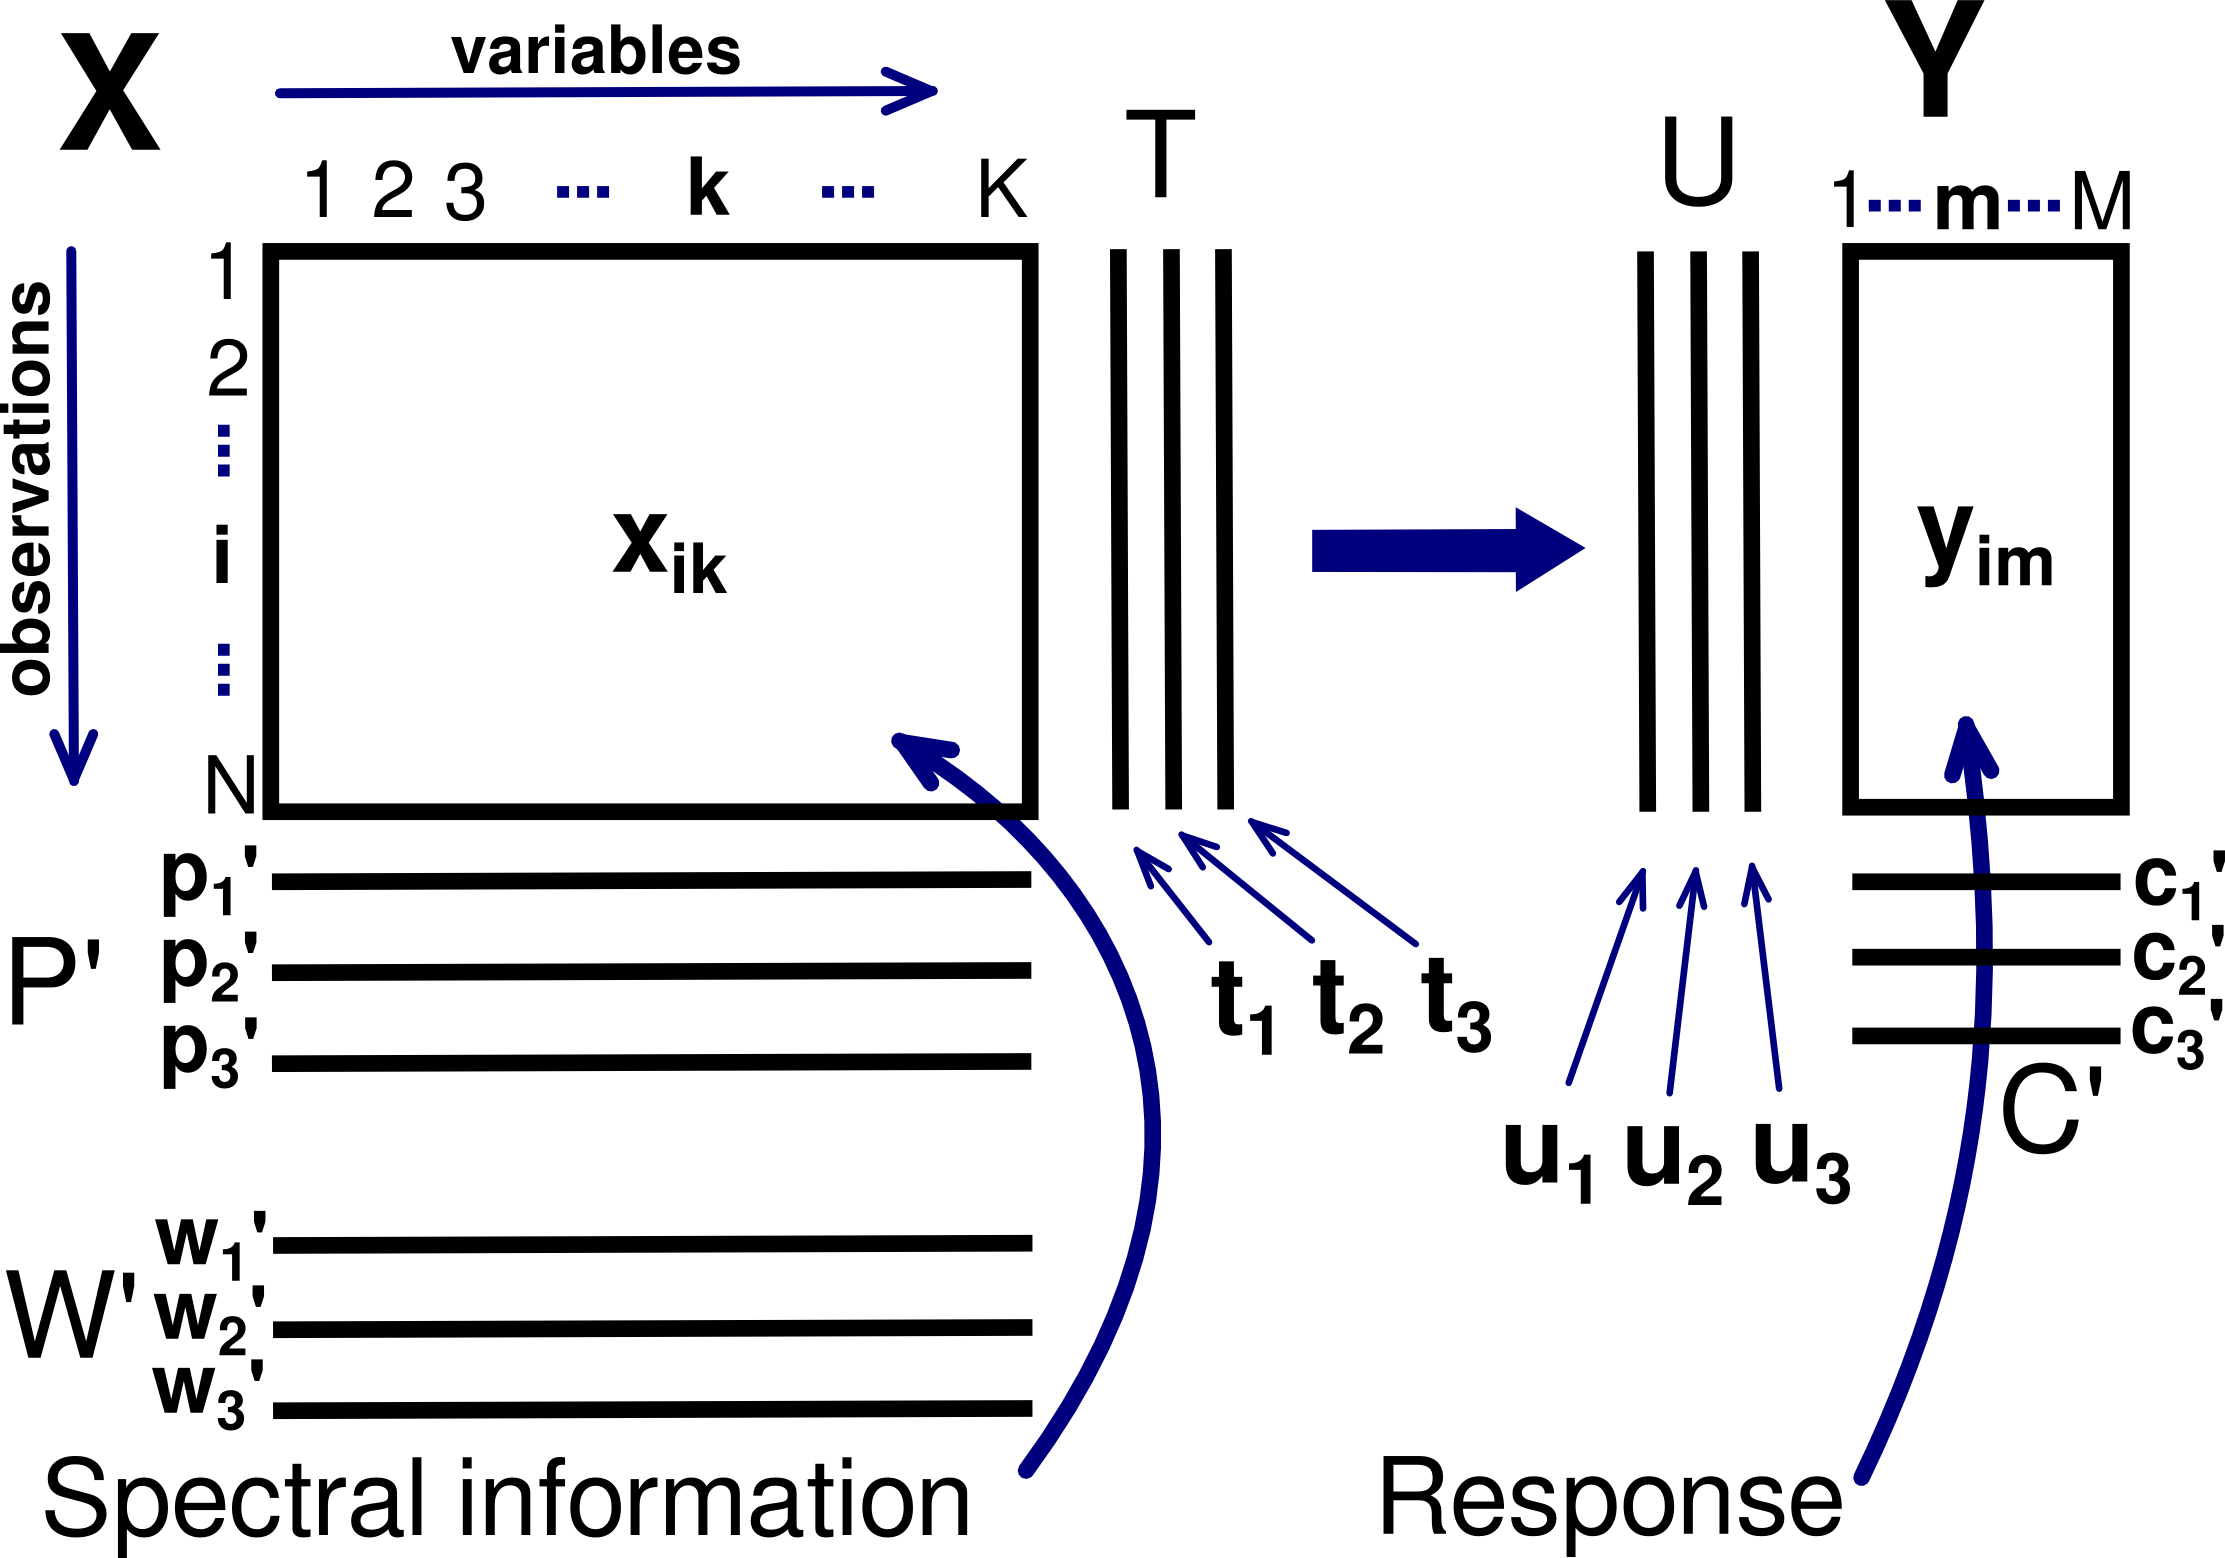
\includegraphics[width=3.75in]{figs/mva/01-bilinear.png}
\end{center}
\caption
      [Canonical Example of a Bilinear Modeling Problem.]{
  {\bf Canonical Example of a Bilinear Modeling Problem.}
  \\
  Illustration of a data matrix $\mathbf{X}$ and a response matrix
  $\mathbf{Y}$, as they are typically used in partial least squares
  modeling problems. In metabolomics applications, the data matrix will
  contain a set of $N$ spectra, each having $K$ variables. For supervised
  modeling problems, each observation in the data matrix is paired with a
  corresponding row in the response matrix that holds either continuously
  varying outputs or binary class memberships. The data are then decomposed
  into a small number of score vectors ($\mathbf{t}$) and loading vectors
  ($\mathbf{p}$), with corresponding weight vectors ($\mathbf{w}$) used
  to transform the observations in $\mathbf{X}$ into scores-space. The
  responses in $\mathbf{Y}$ are similarly decomposed into scores
  ($\mathbf{u}$) and loadings ($\mathbf{c}$). Tick marks denote
  transposition.
}
\label{figure.3.1}
\end{figure}

\section{Multivariate Datasets}

\begin{doublespace}
In the majority of cases, multivariate datasets used in metabolomics take the
form of second-order tensors in $\mathbb{R}^{N \times K}$. More simply, these
datasets are real matrices having $N$ rows and $K$ columns. By convention,
the data are arranged as $N$ observation row vectors of length $K$, where $K$
is referred to as the dimensionality of the dataset (\figref{3.1}{Figure 3.1}).
Typical examples of 1D datasets include sets of \hnmr{} or \cnmr{} NMR spectra
\cite{beckonert:nprot2007,koh:colon2009}, direct-injection mass spectra
(DI-MS, \cite{castrillo:phch2003,southam:anchem2007,zhou:asms2010}), infrared
(IR) and Raman spectra \cite{ellis:analyst2006,cherney:anchem2007}, or
capillary electrophoretograms (CE, \cite{ramautar:trac2006}). This remarkable
diversity of instrumental platforms used in metabolomics is traceable to the
ability of bilinear factorizations such as principal component analysis
(PCA, \cite{jolliffe2002}) and partial least squares (PLS, \cite{wold1993}) to
directly accept these second-order tensors for modeling (vide infra).
\\\\
The dimensionality of a multivariate dataset may be increased by adding another
``mode'', resulting in a third-order (or higher) tensor
($\mathbf{X} \in \mathbb{R}^{N \times K_1 \times K_2}$,
\figref{3.2}{Figure 3.2}). In such cases, the total dimensionality of the
dataset is now the product of the dimensionalities along each mode of the
data tensor (e.g. $K_1 \times K_2$). Third-order tensors are the natural
data structures for sets of two-dimensional observations, including
\hhnmr{}, \hcnmr{} and \hnnmr{} NMR spectra, hyphenated chromatography-mass
spectra (LC-MS, GC-MS), hyphenated electrophoresis-mass spectra (CE-MS), and
hyphenated ion-mobility mass spectra (IM-MS). While third-order data tensors
may hold substantially more chemical information than their second-order
counterparts, they are not directly compatible with bilinear factorization
methods, and they require specialized processing, treatment and modeling
algorithms \cite{lu:ieee2009,lu:pr2011}. As an example, tensors may be
vectorized into matrices \cite{hedenstrom:cils2008} that are suited for
PCA and PLS, but at the cost of lost structural information. Methods such
as uncorrelated multilinear PCA (UMPCA, \cite{lu:ieee2009}), on the other
hand, provide a means of directly decomposing tensors into low-dimensional
spaces while maintaining structural information.
\end{doublespace}

\begin{SCfigure}
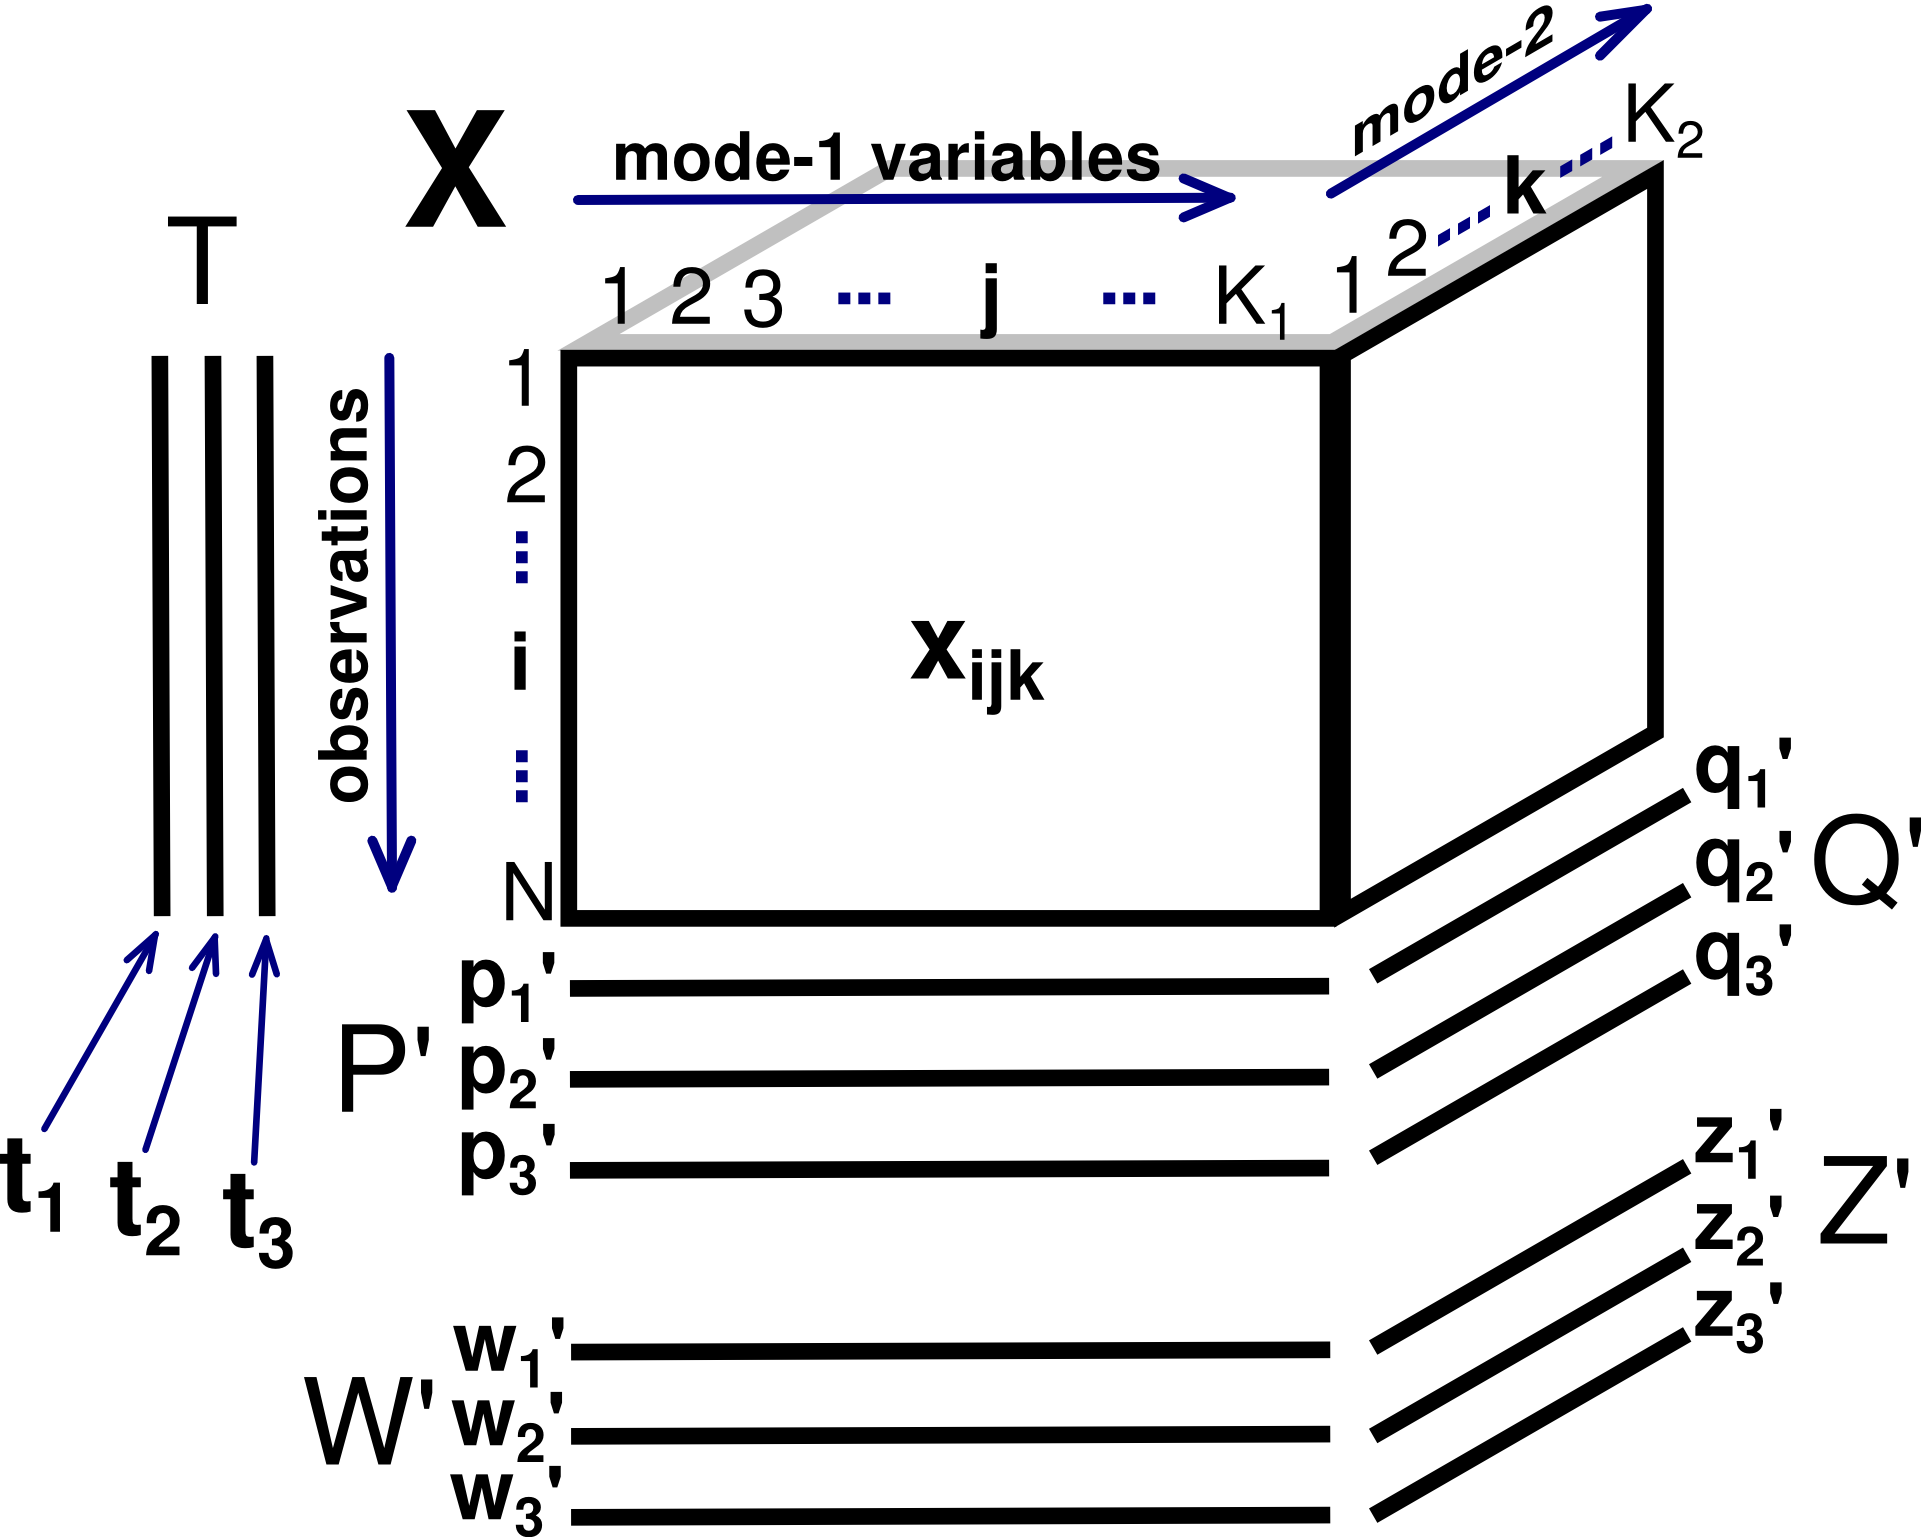
\includegraphics[width=3.25in]{figs/mva/02-trilinear.png}
\caption
      [Canonical Example of an Unsupervised Trilinear Modeling Problem.]{
  {\bf Canonical Example of an Unsupervised Trilinear Modeling Problem.}
  \\
  Illustration of a third-order data tensor $\mathbf{X}$ as may be found in
  multilinear factorization problems. Such data tensors will contain a set
  of $N$ spectra, each having $K_1$ variables along their first mode and
  $K_2$ variables along their second. The data tensor is then decomposed
  into a small number of score vectors ($\mathbf{t}$) and loading vectors
  ($\mathbf{p}$, $\mathbf{q}$), with corresponding weight vectors
  ($\mathbf{w}$, $\mathbf{z}$) used to transform the observations in
  $\mathbf{X}$ into scores-space. Tick marks denote transposition.
}
\label{figure.3.2}
\end{SCfigure}

\begin{figure}[ht!]
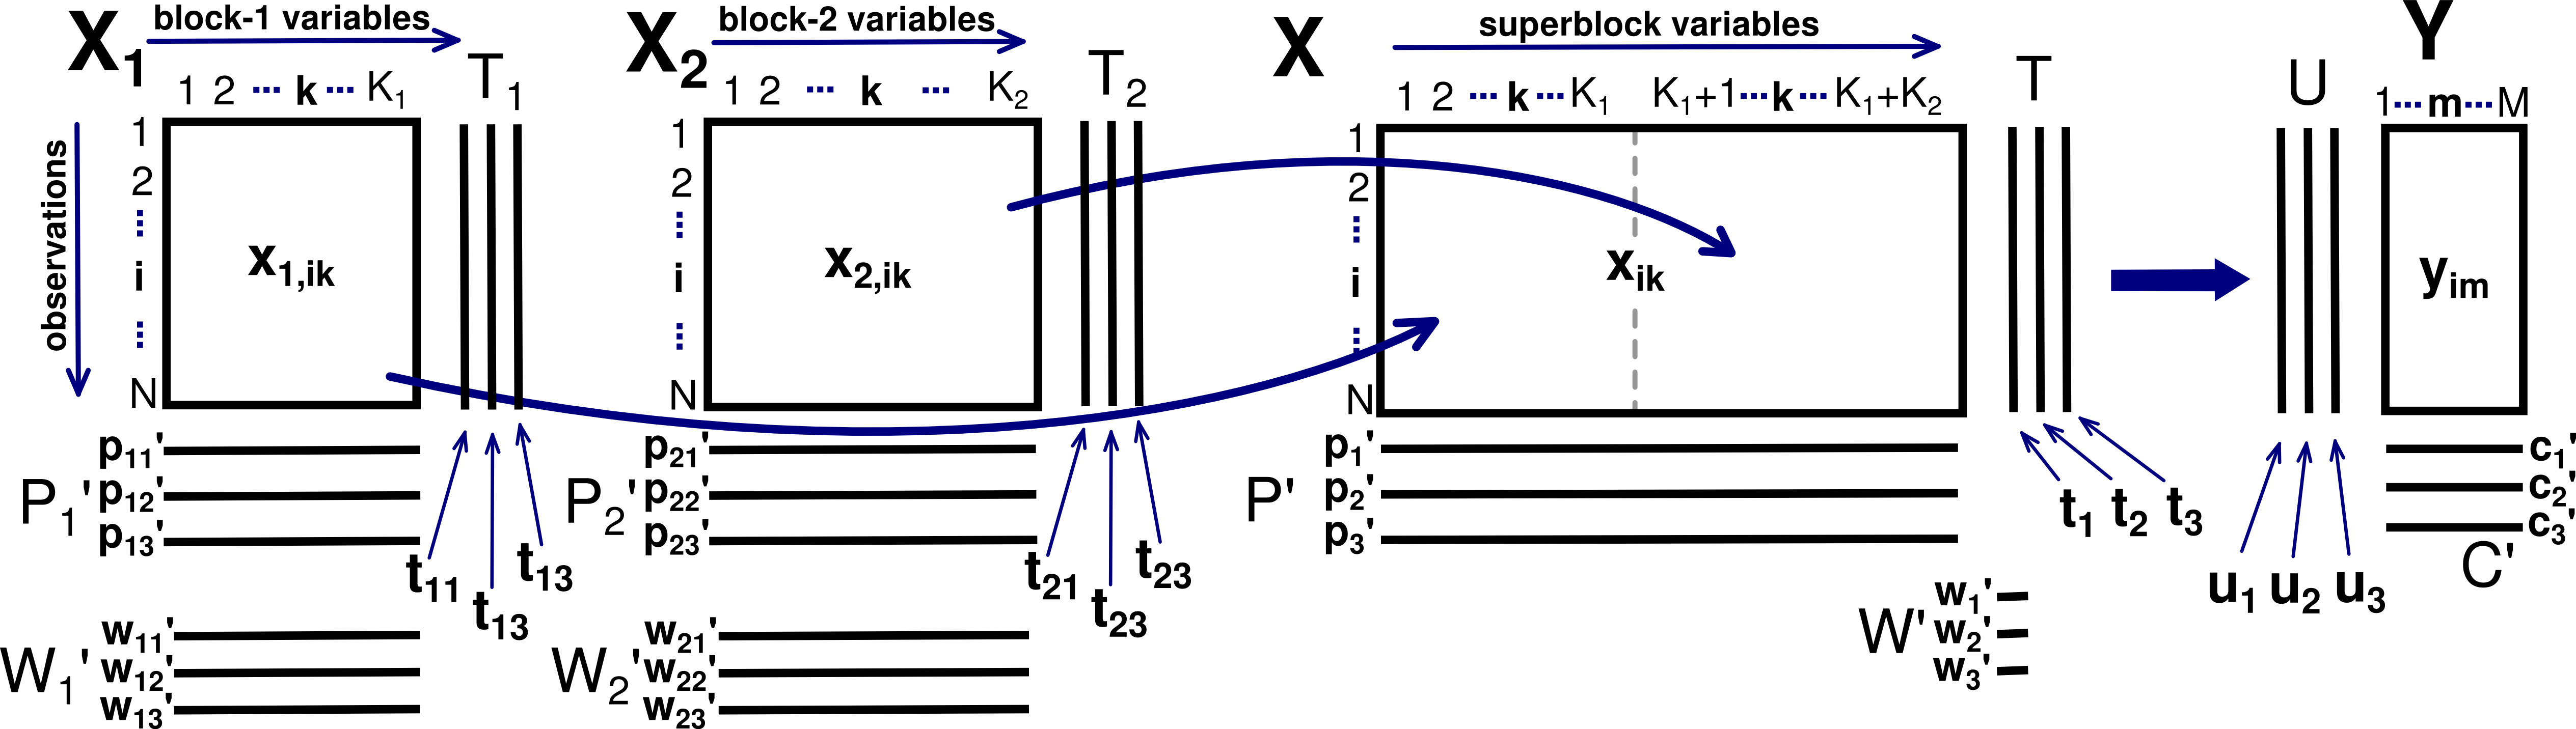
\includegraphics[width=6in]{figs/mva/03-multiblock.png}
\caption
      [Canonical Example of a Multiblock Bilinear Modeling Problem.]{
  {\bf Canonical Example of a Multiblock Bilinear Modeling Problem.}
  \\
  Illustration of a pair of data matrices $\mathbf{X}_1$ and $\mathbf{X}_2$,
  their observation-wise concatenation $\mathbf{X}$, and a response matrix
  $\mathbf{Y}$, as they are typically used in multiblock partial least squares
  modeling problems. In metabolomics applications, each data matrix
  $\mathbf{X}_b$ in the set of $B$ matrices will contain a set of $N$ spectra,
  each having $K_b$ variables. The data are then decomposed into a small number
  of superblock score vectors ($\mathbf{t}$) and superblock loading vectors
  ($\mathbf{p}$), with corresponding superblock weight vectors ($\mathbf{w}$).
  Each individual data matrix is also decomposed into a set of block scores
  ($\mathbf{t}_b$), block loadings ($\mathbf{p}_b$) and block weights
  ($\mathbf{w}_b$). Tick marks denote transposition.
}
\label{figure.3.3}
\end{figure}

\begin{doublespace}
Another mechanism of increasing the information content of datasets entering
into multivariate chemometric models is to collect spectral observations on
two or more complementary instrumental platforms for each sample. In such a
``multiblock'' modeling approach, each data block $\mathbf{X}_b$ contains $N$
$K_b$-variate observations \cite{westerhuis:jchemo1998,smilde:jchemo2003}.
Bilinear methods such as consensus PCA (CPCA), hierarchical PCA and PLS, and
multiblock PLS may then be used to provide information about data variation
that is correlated between data blocks. Recent examples of multiblock modeling
in metabolomics include fusions of near-IR and mid-IR spectra
\cite{bras:cils2005}, \hnmr{} NMR and direct injection electrospray mass
spectra (DI-ESI-MS, \cite{marshall:metab2015}), and observations from multiple
sensors in process control applications \cite{ferreira:jchemo2010}.
\end{doublespace}

\section{Spectral Processing}

\begin{doublespace}
Following the acquisition of experimental data, instrumentation-specific
processing must be applied to transform the data into a suitable set of
real matrices for bilinear modeling, or tensors for multilinear modeling.
Because the majority of data presented herein originated from an NMR
spectrometer, and because NMR spectra present unique challenges to the
analyst during data handling, the following discussions will center around
processing of 1D and 2D NMR datasets.
\end{doublespace}

\subsection{NMR Signals}

\begin{doublespace}
Modern NMR spectrometers effectively acquire a rotating-frame free induction
decay (FID) through the use of quadrature phase detection of the incoming
signal \cite{levitt2008}. This detection method imparts relative phase
information to the time-domain decays by creating an ``in-phase'' signal
component $i(t)$ and a ``quadrature'' component $q(t)$ phased ninety degrees
from $i(t)$. Indirect dimensions of multidimensional NMR experiments are also
collected in quadrature through interleaved acquisition of one-dimensional
decays that have been cosine- and sine-modulated by the indirect-dimension
signals \cite{states:jmr1982}. As a result, each data point in a
$D$-dimensional NMR signal collected in complete quadrature exists in a
hypercomplex space $\mathbb{H}_D$ \cite{schuyler:jmr2013}, which is defined by
a real basis element and $D$ complex basis elements:
\begin{equation}
\Phi_D \equiv \{ 1 \cdot u_1 \cdots u_D \}
\end{equation}
where multiplication by any complex element $u_d$ results in a ninety degree
phase shift in dimension $d$, and the basis elements combine commutatively
under multiplication, as follows:
\begin{align}
u_i u_j =& u_j u_i \\
u_i^2 =& -1
\end{align}

The basis elements in $\Phi_D$ are a generating set for the complete set of
components of the hypercomplex space $\mathbb{H}_D$. For example, in three
dimensions:
\begin{equation}
\Phi_3 = \{ 1, u_1, u_2, u_1 u_2, u_3, u_1 u_3, u_2 u_3, u_1 u_2 u_3 \}
\end{equation}

A scalar in $\mathbb{H}_D$ is then expressed as a linear combination of this
component set. For the three-dimensional example:
\begin{equation}
x = a + b u_1 + c u_2 + d u_1 u_2
  + e u_3 + f u_1 u_3 + g u_2 u_3 + h u_1 u_2 u_3
\end{equation}
or, more generally and succinctly:
\begin{equation}
x = \sum_{\phi \in \Phi_D} x \{ \phi \} \cdot \phi
\end{equation}
where $x\{\phi\}$ denotes the real coefficient of $x$ that scales the basis
component $\phi$ in $x$. For the above three-dimensional example, the
expression $x\{u_1 u_3\}$ would evaluate to $f$. Finally, the expression of
hypercomplex tensors is formally accomplished by defining each coefficient
as a real tensor of appropriate size, like so:
\begin{equation}
x \{ \phi \} \in \mathbb{R}^{k_1 \cdots k_K} \quad \forall \phi \in \Phi_D
\end{equation}
where $K$ is the number of modes of the tensor. The above equation may be
compactly written as $\mathbb{H}_D^{k_1 \cdots k_K}$. Any scalar
in $\mathbb{H}_D$ -- and therefore any data point in a $D$-dimensional
quadrature-complete NMR dataset -- shall require $2^D$ real coefficients
in order to be completely determined. While the hypercomplex
algebras $\mathbb{H}_0$ and $\mathbb{H}_1$ are isomorphic to the real 
($\mathbb{R}$) and complex ($\mathbb{C}$) numbers, respectively, $\mathbb{H}_2$
and $\mathbb{H}_3$ are {\it not} isomorphic to the quaternions and octonions,
as the latter are noncommutative under multiplication. This hypercomplex
algebra, introduced for partial-component nonuniform subsampling by Schuyler
et al. \cite{schuyler:jmr2013}, provides an elegant formalism for expressing
and handling NMR data.
\\\\
Mathematically, 1D NMR free induction decays are described by the following
commonly used parametric signal model:
\begin{equation}
f(t) = \sum_{m=1}^M \alpha_m \exp\left\{
  u_1 (\omega_m t + \theta_m) - \rho_m t
  \right\}
\end{equation}
where $\alpha_m$, $\omega_m$, $\theta_m$ and $\rho_m$ represent the amplitude,
frequency, phase error and decay rate of the $m$-th damped complex exponential
in the model $f(t)$. Using the above formalism for hypercomplex tensors, this
signal model is trivially extended to any number of dimensions by multiplying
in a modulation term for each dimension:
\begin{equation}
f(\mathbf{t}) = \sum_{m=1}^M \alpha_m \prod_{d=1}^D \exp\left\{
  u_d (\omega_{m,d} t_d + \theta_{m,d}) - \rho_{m,d} t_d
  \right\}
\end{equation}

For example, a 2D FID may be modeled as follows:
\begin{equation}
f(t_1, t_2) = \sum_{m=1}^M \alpha_m \exp\left\{
  u_1 (\omega_{m,1} t_1 + \theta_{m,1}) +
  u_2 (\omega_{m,1} t_2 + \theta_{m,2}) -
  \rho_{m,1} t_1 - \rho_{m,2} t_2
  \right\}
\end{equation}

In short, NMR free induction decays may be treated as sums of damped
hypercomplex exponentials. While it is possible to directly parameterize
$f(\mathbf{t})$ using either maximum likelihood estimation
\cite{chylla:jbnmr1995,chylla:jbnmr1998,chylla:anchem2011} or Bayesian
model selection and estimation
\cite{bretthorst:jmr1990a,
      bretthorst:jmr1990b,
      bretthorst:jmr1990c,
      chylla:jbnmr1993}, this chapter will focus on the soft modeling of
multiple NMR spectra using bilinear matrix factorizations. However, the above
parametric description of NMR data is useful in understanding various
processing tasks required by these hypercomplex tensors.
\end{doublespace}

\subsection{Time-domain Processing}

\begin{doublespace}
Processing of acquired NMR data is broken into two stages, where time-domain
data is manipulated, transformed into the frequency domain, and further
processed using frequency-domain functions \cite{hoch1996}.
The most routinely used time-domain NMR processing function -- and the first
to be applied during processing -- is referred to as apodization, where the
free induction decay tensor is multiplied point-wise by a window function
$w(\mathbf{t})$ that varies over $\mathbf{t}$. Multiplication by this window
function serves several purposes, including noise reduction, resolution
enhancement, shaping of individual resonances and removal of $\sin(x)/x$
truncation artifacts in the frequency domain. During apodization, it is also
common practice to selectively scale the first collected data point in an
attempt to reduce later frequency-domain baseline distortions
\cite{stoch:jmr2005,ebel:jmr2006}.
\\\\
Following apodization, one or more dimensions of the time-domain NMR data may
be extended with zeros, a process known as zero-filling. Doubling of the number
of data points by zero-filling is a well-established method of increasing both
the digital resolution and the signal-to-noise ratio (SNR) of an NMR signal,
and further zero-filling only achieves a smoother interpolation of signals in
the frequency domain \cite{ebel:jmr2006}. A final use of zero-filling is to
augment the size of a given dimension into a power of two, enabling the use of
a fast Fourier transform (FFT, \cite{cooley:mcomp1965}) in lieu of the slower
discrete Fourier transform (DFT) to move the data into the frequency domain.
\end{doublespace}

\begin{figure}[ht!]
\includegraphics[width=6in]{figs/mva/04-windows.png}
\caption
      [Commonly Applied Window Functions.]{
  {\bf Commonly Applied Window Functions.}
  \\
  Window functions ({\bf A}) produced from a 3.0 Hz exponential (red), a
  3.0 Hz Gaussian (green), and a squared-cosine (blue). Discrete Fourier
  transforms of the window functions in ({\bf A}), zoomed around the first
  few (low frequency) data points, are shown in ({\bf B}). Multiplication of
  a time-domain signal by a given window function in ({\bf A}) results in a
  convolution of its frequency-domain counterpart with the impulse response
  in ({\bf B}). Frequency values in ({\bf B}) are normalized.
}
\label{figure.3.4}
\end{figure}

\subsection{Frequency-domain Processing}

\begin{doublespace}
When NMR free induction decays have been digitized on a grid of uniformly
spaced time-domain points, the most convenient method of transforming them
into the frequency domain is the discrete Fourier transform (DFT,
\cite{bretthorst:cmr2008,schuyler:jmr2013}). Using the introduced formalism for
hypercomplex NMR data, the DFT along dimension $d$ of a time-domain vector
$\mathbf{f} \in \mathbb{H}_D^N$ is defined\footnote{
  For succinctness, the set of integers from $\alpha$ to $\beta$
  shall be denoted as $\mathbb{Z}_\alpha^\beta$, i.e.
  $\mathbb{Z}_\alpha^\beta \equiv \{
   i \mid i \in \mathbb{Z} \wedge \alpha \le i \le \beta
   \}$
} as:
\begin{equation}
\mathbf{s}_k = \frac{1}{\sqrt{N}} \sum_{n=0}^{N-1}
  \exp\left\{ -2 \pi u_d \frac{n k}{N} \right\}
  \mathbf{f}_n
  \quad \forall k \in \ints{0}{N-1}
\end{equation}
which is a linear transformation
$\mathcal{F}_d : \mathbb{H}_D^N \to \mathbb{H}_D^N$. Discrete Fourier
transformation of multidimensional NMR data along one dimension requires the
application of $\mathcal{F}_d$ to every $d$-mode vector of the hypercomplex
tensor, and full Fourier transformation requires such an operation along each
mode of the tensor. Discrete Fourier transformation is computationally
efficient when using the FFT, and requires no prior knowledge about the
frequency content of the data. However, when only a subset of data points
have been collected from a uniform Nyquist grid, as is the case during
nonuniform sampling (NUS), the DFT is a sub-optimal estimator of frequency
content, and other non-Fourier methods of transformation are required
\cite{bretthorst:cmr2008,mobli:pnmrs2014}.
\\\\
Once transformed into the frequency domain, NMR spectra require a phase
correction processing step, in which a phase factor $\Theta(\omega)$ is
multiplied point-wise with the data to correct for phase errors
(i.e. $\theta_{m,d}$ terms in $f(\mathbf{t})$) in the data. For example, a
1D phase-factor along dimension $d$ would have the following form:
\begin{equation}
\Theta(\omega) = e^{ -u_d \theta(\omega) }
\end{equation}

Ideally, the detected time-domain free induction decays would arrive in-phase
with respect to the receiver, and fine tuning of acquisition parameters can
often accomplish this \cite{chylla:jbnmr1998}.
However, variations in receiver phase, dead time
between the transmit and receive gating circuits, and delays arising from
analog and digital filtering can all introduce phase errors. These phase
errors mix the in-phase and quadrature components of the hypercomplex signal,
and produce a mixture of desirable absorptive spectral lines and broad
dispersive lines between the real and imaginary components of each data point.
Unmixing of these absorptive and dispersive contributions to the real spectral
component involves the identification of the phase error $\theta(\omega)$, an
expansion of phase error terms as powers of $\omega$:
\begin{equation}
\theta(\omega) = \theta_0 + \theta_1 \omega + \theta_2 \omega^2 + \dots
\end{equation}

Realistically, phase errors higher than first-order are not observed in modern
NMR spectra, and phase correction rests on the determination of a zero-order
phase error ($\theta_0$) and a first-order phase error ($\theta_1$) in each
dimension. This determination may be performed manually, through
software-interactive adjustment of zero- and first-order corrections by the
analyst. However, manual phase correction is generally too time-consuming in
the case of chemometric studies, where there are tens to hundreds of spectra
to correct. In that case, the task of phase correction is handed to any number
of automated routines that correct each spectrum individually. Spectra may be
automatically phase-corrected by maximization of the most negative absorptive
data point \cite{siegel:aca1981}, analysis of the absorption-versus-dispersion
\cite{craig:jmr1988} or symmetry \cite{heuer:jmr1991} characteristics of
spectral lines, baseline optimization \cite{brown:jmr1989} or entropy
minimization \cite{chen:jmr2002}, to name a few. It is important to note that,
when the ultimate fate of the spectral data is multivariate analysis, the
phase-correction of each spectrum in isolation is wasteful of information that
is available from treating the dataset as an ensemble \cite{worley:cils2014},
as phase differences {\it between} spectra non-linearly affect both line shapes
and baseline, possibly emphasizing spectral details that contain no
chemically or biochemically relevant information.
\end{doublespace}

\section{Statistical Treatment}

\begin{doublespace}
The properties of the bilinear factorizations commonly applied in metabolomics
dictate that processed data tensors be treated by one or more operations before
they are suitable for modeling. These statistical treatments generally aim to
either reduce the dimensionality of the data tensor (i.e. binning and variable
selection) or increase the self-consistency of observations and variables
(i.e. alignment, normalization and scaling). Treatment operations are usually
instrumentation-agnostic, as the data at this stage of handling almost always
fall into one of the general structures outlined in
\hyperlink{section.3.2}{Section 3.2}.
\end{doublespace}

\begin{figure}[ht!]
\includegraphics[width=6in]{figs/mva/05-binning.png}
\caption
      [Example Bin Region Selection Results.]{
  {\bf Example Bin Region Selection Results.}
  \\
  Simulated \hnmr{} NMR spectra of citrate in 20 samples having pH values
  normally distributed around $6.0 \pm 0.05$ pH units, binned using uniform
  ({\bf A}, {\bf B}), optimized ({\bf C}, {\bf D}) and adaptive-intelligent
  ({\bf E}, {\bf F}) algorithms. Results of bin region integration are shown
  in the bottom panels.
}
\label{figure.3.5}
\end{figure}

\subsection{Binning}

\begin{doublespace}
Because the chemical shifts of \hnmr{} nuclei depend strongly on temperature,
pH, ionic strength, and several other factors that affect their electronic
environment, spectral datasets acquired for NMR metabolic fingerprinting
suffer from imprecision in \hnmr{} chemical shifts between observations.
This chemical shift imprecision, known as a problem of imperfect correspondence
among variables in $\mathbf{X}$ \cite{aberg:abc2009}, decreases the reliability
and interpretability of multivariate bilinear models (e.g. PCA, PLS) trained
directly on full-resolution spectral data in $\mathbf{X}$. Similar errors in
correspondence may also occur in chromatographic datasets, where small drifts
in retention time arise from instrumental instability, analyte interactions,
and fluctuations in mobile phase and stationary phase composition
\cite{nielsen:jchrom1998}. The traditional method of mitigating imperfect
variable correspondence in a data matrix is to partition the original set
of variables into a smaller set of regions, referred to as bins, and
to integrate each bin to yield a data matrix having reduced dimensionality.
\\\\
While binning masks variable mis-correspondence, filters incoherent
instrumental noise, and achieves substantial dimensionality reduction, it often
hides potentially significant variation in low-intensity resonances nearby
strong signals. If bin regions are specified with a uniform size, binning is
nearly guaranteed to split signals or spectral features into multiple bins,
resulting in undesirable multicollinearities within the reduced variable set.
Optimized binning \cite{sousa:cils2013} attempts to avoid dividing signals
between bins by adjusting uniform bin boundaries into local minima of the
data matrix mean, $\langle\mathbf{X}\rangle$. However, because optimized
binning begins with a uniform bin set, its practical ability to minimize peak
splitting is limited. More complex methods of region identification use either
peak detection \cite{davis:cils2007} or recursive subdivision
\cite{demeyer:anchem2008} in order to define a more optimal bin set without
relying on uniform bin boundaries.
\end{doublespace}

\begin{figure}[hb!]
\includegraphics[width=6in]{figs/mva/06-align.png}
\caption
      [Example \emph{i}COshift Alignment Results.]{
  {\bf Example \emph{i}COshift Alignment Results.}
  \\
  Full-resolution ({\bf A}) and interval correlation-optimized shifting
  ({\it i}COshift) aligned ({\bf B}) 1D \hnmr{} NMR spectra from a chemometric
  study of brewed coffee roasts. Spectral alignment was performed such that
  each observation was shifted to maximize correlation with its respective
  group mean. Spectral color indicates the observation index.
}
\label{figure.3.6}
\end{figure}

\subsection{Alignment}

\begin{doublespace}
Binning capably masks variability in signal positions and provides an effective
means of dimensionality reduction, but it also results in a drastic loss of
fine spectral information, as nearby distinct spectral features have been
integrated together in the binning process. When full spectral resolution is
required during model training and interpretation, the correspondence problem
in NMR and chromatographic datasets may be alternatively addressed by signal
alignment methods. The most commonly applied alignment algorithms rely on
either a warping transformation
\cite{nielsen:jchrom1998,
      forshed:aca2003,
      wu:jcim2006} or linear shifts
\cite{veselkov:anchem2009,
      savorani:jmr2010,
      tomasi:jchrom2011} to bring individual variables of each observation
into alignment with a reference observation, which is usually the mean of
the data. Warping during alignment is more applicable in situations where
a linear dependence between variable index (e.g. retention time) and peak
width is expected. In contrast, shift-based alignment preserves peak width,
which is ideal for spectroscopic datasets. Like binning, all alignment
algorithms must first subdivide the variable set into regions that are then
individually warped or shifted, and considerations similar to those in
binning apply equally well during alignment region selection.
\end{doublespace}

\subsection{Normalization}

\begin{doublespace}
Despite the quantitative nature of most spectroscopic platforms, chemometric
samples exhibit variable total analyte concentrations due to variations in
sample preparation, instrument stability, or even the samples themselves.
These ``dilution errors'' are especially common in metabolomics experiments
using samples of biofluids such as urine, where total concentrations may vary
several orders of magnitude. To ensure spectral intensities in a data tensor
are directly comparable across each observation, normalization is applied to
the tensor \cite{worley:cmb2013}. The most common normalization method used in
chemometrics is unit-integral or constant-sum (CS) normalization, where each
observation is scaled such that its total integral is unity
\cite{craig:anchem2006}. CS normalization does more harm that good, however,
as it introduces false correlations between variables and poorly tolerates
large disparities in intensities between each observation.
\\\\
In an attempt to overcome the drawbacks of CS normalization, Dieterle et al.
introduced probabilistic quotient (PQ) normalization, in which the median
normalization quotient between all corresponding data points is used as an
estimator of the true dilution factor \cite{dieterle:anchem2006}. Shortly
after, a method of normalization based on intensity histogram matching (HM)
was proposed as an alternative to PQ normalization, taking cues from image
processing algorithms \cite{torgrip:metab2008}. Based on their ability to
more accurately recover true dilution factors, both PQ and HM normalization
were reported to outperform CS normalization on real and simulated \hnmr{}
NMR metabolomics data matrices. Finally, while more commonly applied to
IR spectroscopic data, standard normal variate (SNV) and its mathematical
cousin, multiplicative scatter correction (MSC) are also candidate methods
for normalizing data tensors produced by NMR and other spectroscopic
platforms \cite{fearn:cils2009}.
\end{doublespace}

\begin{SCfigure}
\includegraphics[width=3.25in]{figs/mva/07-scaling.png}
\caption
      [Effects of Scaling Noisy Synthetic Spectra.]{
  {\bf Effects of Scaling Noisy Synthetic Spectra.}
  \\
  ({\bf A}) Set of 40 synthetic spectra containing two Lorentzian signals. The
  first set of signals at 7.0 ppm have normally distributed intensities of
  $20 \pm 0.5$ absolute units, and the second set at 3.0 ppm are divided into
  two sets of intensities, the first normally distributed around $25 \pm 0.5$
  units and the second around $30 \pm 0.5$ units.
  \\
  ({\bf B}) The same set of synthetic spectra after subtraction of the sample
  mean of the data matrix. The two sets of intensities at 3.0 ppm now appear
  markedly different after centering.
  \\
  ({\bf C}) The set of synthetic spectra after unit variance (UV) scaling,
  illustrating the strong noise amplification effect of the UV method.
  \\
  ({\bf D}) The set of synthetic spectra after Pareto scaling, in which noise
  amplification is reduced relative to UV scaling.
}
\label{figure.3.7}
\end{SCfigure}

\subsection{Scaling}

\begin{doublespace}
Because bilinear factorization methods such as PCA and PLS generate models
based on the eigenstructure of the covariance matrices of $\mathbf{X}$ and
$\mathbf{Y}$ (vide infra), they are sensitive to the magnitudes of individual
variables in those matrices. Variables with greater intensity -- and therefore
greater variance -- in a data matrix will draw the attention of these methods,
resulting in an unequal weighting of variable importance during model training
\cite{jolliffe2002,smilde:anchem2005,vandenberg:bmcg2006}. As a consequence,
analysts commonly apply one or more scaling transformations to their data prior
to modeling. The simplest and most pervasive method, referred to as Unit
Variance (UV) scaling, centers each variable with respect to its mean and
scales by its standard deviation, like so:
\begin{equation}
\tilde{x}_{nk} = \frac{x_{nk} - \bar{x}_k}{s_k}
\end{equation}
where $\widetilde{\mathbf{X}}$ is the scaled data matrix, $\bar{x}_k$ is the
sample mean of the $k$-th variable over all $N$ observations, and $s_k$ is the
corresponding sample standard deviation. Subtraction of the sample mean
facilitates the identification of differences between observations, and
scaling by the sample standard deviation equally weights every variable
in $\mathbf{X}$. When data are UV-scaled, methods that normally analyze
covariance eigenstructure will instead rely on {\it scale-invariant}
correlations between variables. Although UV scaling achieves an equal weighting
of all variables entering into PCA or PLS, it amplifies the weight of noise
variables relative to that of signal variables, resulting in decreased model
utility and reliability \cite{hoefsloot:jchemo2006}. Pareto scaling applies a
less aggressive scaling than UV by retaining partial covariance between
variables in an attempt to reduce this noise amplification:
\begin{equation}
\tilde{x}_{nk} = \frac{x_{nk} - \bar{x}_k}{\sqrt{s_k}}
\end{equation}

A more advanced scaling method that avoids noise amplification uses a maximum
likelihood scaling transformation (MALS, \cite{hoefsloot:jchemo2006}) that
accounts for the estimated distribution of noise in $\mathbf{X}$. Other forms
of scaling have been developed that emphasize various desirable features in
a data structure. For example, {\it va}riable {\it st}ability (VAST) scaling
multiplies each element by the coefficient of variation of its variable in
order to focus on highly stable spectral features:
\begin{equation}
\tilde{x}_{nk}
 = \frac{x_{nk} - \bar{x}_k}{s_k} \cdot
   \frac{\bar{x}_k}{s_k}
\end{equation}

The alternative level scaling method scales data elements by their sample mean,
effectively focusing later analyses on changes in relative magnitude:
\begin{equation}
\tilde{x}_{nk} = \frac{x_{nk} - \bar{x}_k}{\bar{x}_k}
\end{equation}

However, both VAST and level scaling have a more limited scope of
application than the general UV, Pareto and MALS methods described above, as
they yield optimal transformations only on data structures containing the
features they aim to accentuate. For example, VAST scaling is not suited for
data tensors that contain large variation between experimental groups, unless
further steps are taken to VAST-scale on a (supervised) per-group basis.
\\\\
A special case for scaling occurs during multiblock modeling when two or more
data blocks contain differing variable counts. In these situations, data blocks
having more variables would acquire a larger effective weight during model
training. For example, joint modeling of full-resolution \hnmr{} NMR data
($K \approx 10^3$) and mass spectral data ($K \approx 10^5$) would result in
a weighting of MS variables by a factor of ten relative to NMR variables. To
achieve equal block weighting, the variables of each block must be scaled by
the square root of the number of block variables:
\begin{equation}
\tilde{\tilde{x}}_{bnk} = \frac{\tilde{x}_{bnk}}{\sqrt{K_b}}
\end{equation}
where the second tilde indicates block scaling in addition to any standard
scaling (e.g. UV, Pareto) that may have been applied. When all data blocks
contain analyte concentrations instead of raw spectral variables, range
scaling may be applied prior to block scaling to remove instrumental response
factors and transform all concentrations into relative values
\cite{smilde:anchem2005}:
\begin{equation}
\tilde{x}_{bnk}
 = \frac{x_{bnk} - \bar{x}_{bk}}
        {\max_n(x_{bnk}) - \min_n(x_{bnk})}
\end{equation}

Range scaling holds intuitive appeal for multiblock modeling of concentration
data, but its application to other kinds of datasets is ill-advised, as it
suffers from similar noise amplification problems as UV scaling.
\end{doublespace}

\subsection{Variable Selection}

\begin{doublespace}
Due to the expense of sample preparation and data acquisition in metabolomics
studies, a strong temptation exists to retain all observed variables during
multivariate analyses \cite{kjeldahl:jchemo2010}. Because variables are scaled
to equal (or nearly equal) weight prior to modeling, this practice produces
multivariate models that suffer in both predictive ability and general
reliability. In short, only variables that are truly relevant to the chemical
system under study should be included during modeling. To that end,
conservative manual removal of irrelevant variables based on spectroscopic
and biochemical domain knowledge is often performed in metabolomics. \hnmr{}
NMR datasets, for instance, nearly always contain highly varying signals from
solvents, buffers, and chemical shift reference compounds, all of which may
confound or overshadow relevant sources of variation. Variables containing
such signals, as well as signal-free variables that only contain instrumental
noise, are excellent candidates for manual variable selection. More
computationally intensive methods of variable selection, including support
vector machine recursive feature elimination (SVM-RFE), genetic algorithms
(GA), random forests (RF) and bootstrapping have also been developed to more
aggressively select variables from multivariate data structures
\cite{lin:metab2011,wongravee:anchem2009}. While it is important to retain
only relevant variables for modeling, an over-aggressive variable selection
is equally detrimental, as it leads to over-fit models that may fail to
tolerate subsequent outlying observations.
\end{doublespace}

\section{Modeling}

\begin{doublespace}
The most widely applied modeling methods in metabolomics -- namely principal
component analysis, partial least squares and orthogonal projections to latent
structures (OPLS, \cite{trygg:jchemo2002}) -- fall within a class of methods
known as bilinear matrix factorizations. The general form of a bilinear matrix
factorization is:
\begin{equation}
\mathbf{X} = \mathbf{T} \mathbf{P}^T + \mathbf{E}
\end{equation}
where the data matrix $\mathbf{X} \in \mathbb{R}^{N \times K}$ is approximated
by the product of two matrices, $\mathbf{T} \in \mathbb{R}^{N \times A}$ and
$\mathbf{P} \in \mathbb{R}^{K \times A}$, which are referred to as ``scores''
and ``loadings'', respectively. The matrix
$\mathbf{E} \in \mathbb{R}^{N \times K}$ holds any variation in $\mathbf{X}$
that is not captured by the scores and loadings. To understand how such a
factorization may be used to approximate a data matrix, it is instructive to
consider the product of scores and loadings in vector form:
\begin{equation}
\mathbf{X} = \sum_{a=1}^A \mathbf{t_a} \mathbf{p_a}^T + \mathbf{E}
\end{equation}
where $\mathbf{t_a}$ and $\mathbf{p_a}$ are the $a$-th columns of the score
and loading matrices, respectively. In other words, the data matrix is
approximated by a set of $A$ rank-1 matrices that are constructed by the
outer products of each pair of scores and loadings. Because $A$ is commonly
much less than either $N$ or $K$, these bilinear factorizations are also
referred to as low-rank approximations of their data matrices.
\end{doublespace}

\begin{figure}[ht!]
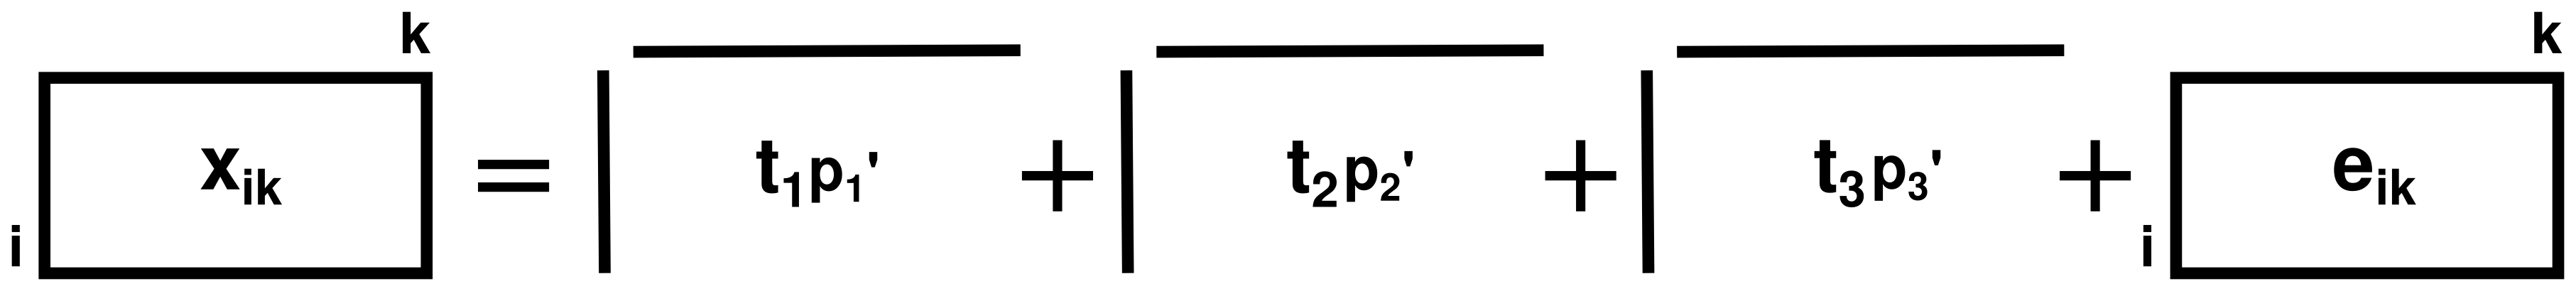
\includegraphics[width=6in]{figs/mva/08-lowrank.png}
\caption
      [Example Three-component Bilinear Low-rank Approximation.]{
  {\bf Example Three-component Bilinear Low-rank Approximation.}
  \\
  Depiction of a three-component bilinear low-rank approximation
  $\mathbf{T} \mathbf{P}^T$ of a data matrix $\mathbf{X}$ having
  residuals $\mathbf{E}$, with each outer product of the approximation
  broken out.
}
\label{figure.3.8}
\end{figure}

\begin{doublespace}
It is important to note that nearly every data matrix modeled by equation
(3.20) in metabolomics contains far fewer observations than variables
(i.e. $N \ll K$) \cite{worley:cmb2013}. In this situation, there are infinitely
many solutions to the equation that yield the same error $\mathbf{E}$. This is
easily demonstrated by multiplying the scores and loadings by an orthonormal
matrix $\mathbf{R} \in \mathbb{R}^{A \times A}$:
\begin{align}
\mathbf{X}
 =& \: \hat{\mathbf{T}} \hat{\mathbf{P}}^T + \mathbf{E}
\nonumber \\
 =& \: \mathbf{T} \mathbf{R} \mathbf{R}^T \mathbf{P}^T + \mathbf{E}
\nonumber \\
 =& \: \mathbf{T} \mathbf{P}^T + \mathbf{E}
\end{align}
where $\hat{\mathbf{T}} = \mathbf{T} \mathbf{R}$ and
$\hat{\mathbf{P}} = \mathbf{P} \mathbf{R}$. A similar expansion of the solution
set may be accomplished by multiplying the scores by a diagonal $A \times A$
matrix, and multiplying the loadings by the inverse of the same diagonal
matrix. This equivalence of an infinite number of solutions to equation
(3.20), known as the problems of rotational and scale ambiguity, is solved by
placing constraints on the values that scores and loadings may take
\cite{dejuan:aca1997,jolliffe2002}. The choice of constraints defines a
particular bilinear factorization method as unique, and determines what
kind of information is sought from a data matrix using that method.
\end{doublespace}

\subsection{Principal Component Analysis}

\begin{doublespace}
In principal component analysis (PCA), which exactly follows equation 3.20,
the loading vectors in $\mathbf{P}$ are constrained to be an orthonormal basis
set. More precisely, the loadings produced by PCA are not just any orthonormal
basis, but are in fact the first $A$ eigenvectors of the sample covariance
matrix $\mathbf{X}^T \mathbf{X}$. In chemometrics, the most commonly used
algorithm for constructing PCA models is nonlinear iterative partial least
squares (NIPALS, \cite{geladi:aca1986}):
\end{doublespace}

\begin{algorithm}[H]
\caption{NIPALS Algorithm for PCA}
\label{algorithm.3.1}
\begin{algorithmic}[1]
\REQUIRE $\mathbf{X} \in \mathbb{R}^{N \times K}$
\ENSURE $\mathbf{t} \in \mathbb{R}^N$, $\mathbf{p} \in \mathbb{R}^K$
\STATE $\mathbf{t}^{(0)} \sim U_{N \times 1}$ \COMMENT{
  $\mathbf{t}$ may also be initialized to a column of $\mathbf{X}$
}
\STATE $k \gets 1$
\REPEAT
  \STATE $\mathbf{p}^{(k)} \propto \mathbf{X}^T \mathbf{t}^{(k-1)}$
  \STATE $\mathbf{t}^{(k)} \gets \mathbf{X} \mathbf{p}^{(k)}$
  \STATE $k \gets k + 1$
\UNTIL{
  $\frac{\| \mathbf{t}^{(k)} - \mathbf{t}^{(k-1)} \|_2}
        {\| \mathbf{t}^{(k-1)} \|_2} < \varepsilon$
}
\end{algorithmic}
\end{algorithm}

\begin{SCfigure}
\includegraphics[width=3.25in]{figs/mva/09-pca.png}
\caption
      [Principal Components of Synthetic Bivariate Data.]{
  {\bf Principal Components of Synthetic Bivariate Data.}
  \\
  ({\bf A}) Set of 100 points drawn from a bivariate normal distribution,
  and the corresponding principal components computed by eigendecomposition
  of the points' sample covariance matrix. Bold and thin arrows indicate the
  normalized and un-normalized loadings, respectively.
  \\
  ({\bf B}) Set of 100 points drawn from two bivariate normal distributions
  having different means, where the major source of variation in the data is
  orthogonal to the direction that separates the two groups.
  \\
  ({\bf C}) Set of 100 points drawn from two bivariate normal distributions
  having different means, where the major source of variation is parallel to
  the direction that separates the groups.
}
\label{figure.3.9}
\end{SCfigure}

\begin{doublespace}
where $\gets$ indicates assignment, and $\propto$ indicates normalized
assignment. In others words, the following two statements:
\begin{equation*}
a \propto b \quad \Leftrightarrow \quad a \gets \frac{b}{\|b\|_2}
\end{equation*}
are in fact equivalent. In summary, NIPALS PCA initializes a score vector from
a uniform random distribution, and repeatedly projects the rows and columns of
$\mathbf{X}$ into the score and loading vectors until the scores converge to
a predefined limit $\varepsilon$. By substituting the scores assignment into
the loadings assignment, we arrive at the following iteration equation:
\begin{equation}
\mathbf{p}^{(k)} \gets
 \frac
  {\mathbf{X}^T \mathbf{X} \mathbf{p}^{(k-1)}}
  {\| \mathbf{X}^T \mathbf{X} \mathbf{p}^{(k-1)} \|_2}
\end{equation}
which is the equation for power iteration on $\mathbf{X}^T \mathbf{X}$
\cite{golub2012}. Indeed, the NIPALS algorithm implicitly computes the
dominant eigenvector $\mathbf{p}$ of the $K \times K$ sample covariance
matrix, with a corresponding eigenvalue $\mathbf{t}^T \mathbf{t}$:
\begin{equation*}
\mathbf{X}^T \mathbf{X} \mathbf{p} =
 \left( \mathbf{t}^T \mathbf{t} \right) \mathbf{p}
\end{equation*}

The above algorithm computes a single principal component of $\mathbf{X}$ in
the form of $\mathbf{t}$ and $\mathbf{p}$. In order to compute a second
component, the first component's contributions must be subtracted
from $\mathbf{X}$, a step referred to as ``deflation'':
\begin{equation}
\mathbf{X}' \gets \mathbf{X} - \mathbf{t} \mathbf{p}^T
\end{equation}

Re-application of the NIPALS algorithm to the deflated matrix $\mathbf{X}'$
will then produce the second principal component of the original data matrix
$\mathbf{X}$. This process of power iteration and deflation is repeated until
an optimal number of components $A^\ast$ is reached.
\end{doublespace}

\subsubsection{PCA for Unsupervised Modeling}

\begin{doublespace}
From the algebraic properties of PCA, an intuitive geometric picture may be
constructed (\figref{3.9}{Figure 3.9}). In essence, PCA determines the
directions within a data matrix -- the principal components -- that contain
the greatest sources of variation in that matrix (\figref{3.9}{3.9A}),
where each direction is constrained to be orthogonal to all previous
directions. When observations in $\mathbf{X}$ fall into two or more
experimental groups, they produce different clustering patterns in the PCA
scores $\mathbf{T}$. In cases where the within-group variation in one or
more groups is the major source of variation in $\mathbf{X}$, PCA will fail
to effectively separate the groups in scores space (\figref{3.9}{3.9B}).
However, when the between-group variation significantly contributes to the
total variation in $\mathbf{X}$, the groups will be well-separated
(\figref{3.9}{3.9C}). Thus, PCA is a powerful method of identifying major
trends among variables in a data matrix, as well as general relationships
between observations, and does not bias its results based on class identity.
For a description of methods to quantify separations between experimental
groups in PCA scores space, see \hyperlink{chapter.10}{Chapter 10}.
\end{doublespace}

\subsubsection{PCA for Outlier Detection}

\begin{doublespace}
During data handling, it is common practice to exclude outlying observations,
when warranted by the analysis, in order to ensure relevant information
extraction. In the univariate case, the sample mean $\bar{x}$ and sample
standard deviation $s$ may be estimated from a data vector $\mathbf{x}$,
which may then be standardized into a set of Mahalanobis distances
$\mathbf{d}$:
\begin{equation}
d_n = \frac{x_n - \bar{x}}{s}
 \quad \forall n \in \ints{1}{N}
\end{equation}

These distances in $\mathbf{d}$ may be transformed into $t$ statistics and
compared to critical values of a $t$-distribution using a run plot in order
to visually detect outliers \cite{chambers1983}. In the multivariate case,
the sample mean vector $\bar{\mathbf{x}} \in \mathbb{R}^K$ and the sample
variance-covariance matrix $\mathbf{S} \in \mathbb{R}^{K \times K}$ of the
data matrix $\mathbf{X} \in \mathbb{R}^{N \times K}$ must first be computed:
\begin{align}
\bar{\mathbf{x}} =& \: N^{-1} \sum_{n=1}^N \mathbf{x}_n \\
\mathbf{S} =& \: (N - 1)^{-1} \mathbf{X}^T \mathbf{X}
\end{align}
where $\mathbf{x}_n$ is the $n$-th observation row vector in $\mathbf{X}$.
The set of squared Mahalanobis distances may then be computed as follows
\cite{demaesschalck:cils2000}:
\begin{equation}
d_n^2 =
 (\mathbf{x}_n - \bar{\mathbf{x}}) \mathbf{S}^{-1}
 (\mathbf{x}_n - \bar{\mathbf{x}})^T
 \quad \forall n \in \ints{1}{N}
\end{equation}

Once again, each squared distance may be compared to a critical value from a
$T^2$-distribution to assess the probability that its corresponding observation
is an outlier. The above procedure fails in practice, because the covariance
matrix is severely rank-deficient, and thus non-invertible (i.e. $N \ll K$).
To ensure a stable inversion of the covariance matrix, the data matrix may be
approximated using PCA (i.e. $\mathbf{X} \approx \mathbf{T} \mathbf{P}^T$),
where the number of principal components is less than the rank of the data
matrix. Using the orthonormality property of PCA loadings, squared Mahalanobis
distances may again be obtained from the PCA scores:
\begin{equation}
d_n^2 =
 \mathbf{t}_n
 \left( \frac{\mathbf{T}^T \mathbf{T}}{N - 1} \right)^{-1}
 \mathbf{t}_n^T
 \quad \forall n \in \ints{1}{N}
\end{equation}
where $\mathbf{t}_n$ is the $n$-th row of the scores matrix $\mathbf{T}$.
Because the matrix $\mathbf{T}^T \mathbf{T}$ is diagonal, it is trivially
inverted and calculation of each $d_n^2$ is greatly simplified. Mahalanobis
distances computed using PCA scores are close approximations of their true
values in the original high-dimensional space \cite{demaesschalck:cils2000},
and provide a means of outlier detection in high-dimensional data
(\figref{3.10}{Figure 3.10}). Outliers may be visually identified from scatter
plots of PCA scores (\figref{3.10}{Figure 3.10B}) or from run plots of their
corresponding squared Mahalanobis distances (\figref{3.10}{Figure 3.10C}).
In both cases, the squared Mahalanobis distance is compared to the
$\chi^2$ distribution at a preselected significance $\alpha$ and $A$
degrees of freedom \cite{hotelling:ams1931,worley:abio2013}.
\end{doublespace}

\begin{SCfigure}
\includegraphics[width=3.25in]{figs/mva/10-outlier.png}
\caption
      [PCA for Outlier Testing.]{
  {\bf PCA for Outlier Testing.}
  \\
  ({\bf A}) Set of 40 spectra, generated identically to those in Figure 3.7,
  with the exception of observation 20, which contains an extra Lorentzian
  signal at 6.8 ppm.
  \\
  ({\bf B}) Principal Component Analysis scores plot of the spectral data,
  showing the 68.3\% ($1\sigma$), 95.5\% ($2\sigma$) and 99.7\% ($3\sigma$)
  confidence regions as dashed, thin and bold ellipses, respectively. Point
  colorings indicate relative squared Mahalanobis distances, ranging from blue
  to red as $d^2$ increases.
  \\
  ({\bf C}) Run plot of squared Mahalanobis distances computed from PCA scores
  of the spectral data, again illustrating the one-, two- and three-$\sigma$
  thresholds for outlier detection. Point colorings indicate relative squared
  Mahalanobis distances.
}
\label{figure.3.10}
\end{SCfigure}

\subsubsection{PCA for Multiple Linear Regression}

\begin{doublespace}
Often, a data matrix $\mathbf{X} \in \mathbb{R}^{N \times K}$ is used within
the context of a multiple linear regression to determine a set of regression
coefficients $\mathbf{B} \in \mathbb{R}^{K \times M}$ that best recapitulate
a set of responses $\mathbf{Y} \in \mathbb{R}^{N \times M}$ using the data in
$\mathbf{X}$:
\begin{equation}
\mathbf{Y} = \mathbf{X} \mathbf{B} + \mathbf{E}
\end{equation}

In which case the ordinary least squares (OLS) estimator of the regression
coefficients is obtained from inversion of the normal equations
\cite{draper1998}:
\begin{equation}
\hat{\mathbf{B}} = (\mathbf{X}^T \mathbf{X})^{-1} \mathbf{X}^T \mathbf{Y}
\end{equation}

The OLS regression coefficients $\hat{\mathbf{B}}$ minimize the sum of squares
of the residual matrix, $\frosq{\mathbf{E}}$, and are maximum likelihood
estimates of $\mathbf{B}$ when the errors are independent and identically
normally distributed \cite{draper1998}. However, the fact that $N \ll K$ yet
again makes the matrix $\mathbf{X}^T \mathbf{X}$ non-invertible, forcing the
analyst down a different path. By replacing the data matrix with its PCA
approximation in the regression equation:
\begin{equation}
\mathbf{Y} = \mathbf{T} \mathbf{P}^T \mathbf{B} + \mathbf{E}'
\end{equation}
it is possible to obtain OLS estimates of the regression coefficients:
\begin{align}
\hat{\mathbf{B}}'
 =& \: (\mathbf{P} \mathbf{T}^T \mathbf{T} \mathbf{P}^T)^{-1}
       \mathbf{P} \mathbf{T}^T \mathbf{Y}
 \nonumber \\
 =& \: \mathbf{P} (\mathbf{T}^T \mathbf{T})^{-1} \mathbf{T}^T \mathbf{Y}
 \\
 =& \: \mathbf{P} \hat{\mathbf{G}}
\end{align}
where the matrix $\hat{\mathbf{G}} \in \mathbb{R}^{A \times M}$ is the set of
OLS regression coefficient estimates in PCA scores space:
\begin{equation}
\mathbf{Y} = \mathbf{T} \mathbf{G} + \mathbf{E}'
\end{equation}

By computing the least-squares estimates of the regression coefficients in the
low-dimensional PCA scores space and projecting those estimates into the
original high-dimensional space, this technique of principal component
regression (PCR, \cite{jolliffe2002}) sidesteps the curse of dimensionality
during estimation. Furthermore, the variances of PCR-estimated coefficients
$\hat{\mathbf{B}}'$ are lower than those of the original OLS estimates
$\hat{\mathbf{B}}$. The PCR method will fail to obtain useful estimates,
however, when response-correlated information in the data matrix is not
a major source of variation (cf. \figref{3.9}{Figure 3.9B}). In such cases,
methods such as PLS must be used instead.
\end{doublespace}

\subsection{Partial Least Squares}

\begin{doublespace}
Partial least squares (PLS) approaches the high-dimensional multiple linear
regression problem introduced in equation 3.30 by approximating both
$\mathbf{X}$ \emph{and} $\mathbf{Y}$ using bilinear factorizations
\cite{wold:cils2001}:
\begin{align}
\mathbf{X} =& \: \mathbf{T} \mathbf{P}^T + \mathbf{E} \\
\mathbf{Y} =& \: \mathbf{U} \mathbf{C}^T + \mathbf{G} \\
           =& \: \mathbf{T} \mathbf{C}^T + \mathbf{F} \nonumber
\end{align}
where the last equality indicates that the $\mathbf{X}$-scores are highly
correlated with the $\mathbf{Y}$-scores, and are therefore good predictors
of $\mathbf{Y}$. The most commonly applied algorithm for PLS is once again
NIPALS-based, and is shown below:
\end{doublespace}

\begin{algorithm}[H]
\caption{NIPALS Algorithm for PLS}
\label{algorithm.3.2}
\begin{algorithmic}[1]
\REQUIRE $\mathbf{X} \in \mathbb{R}^{N \times K}$,%
       $\:\mathbf{Y} \in \mathbb{R}^{N \times M}$
\ENSURE $\mathbf{t} \in \mathbb{R}^N$,%
      $\:\mathbf{p} \in \mathbb{R}^K$,%
      $\:\mathbf{w} \in \mathbb{R}^K$,%
      $\:\mathbf{u} \in \mathbb{R}^N$,%
      $\:\mathbf{c} \in \mathbb{R}^M$
\STATE $\mathbf{u} \sim U_{N \times 1}$ \COMMENT{
  $\mathbf{u}$ may also be initialized to a column of $\mathbf{Y}$
}
\REPEAT
  \STATE $\mathbf{w} \propto \mathbf{X}^T \mathbf{u}$
  \STATE $\mathbf{t} \gets \mathbf{X} \mathbf{w}$
  \STATE $\mathbf{c} \gets \tfrac{\mathbf{Y}^T \mathbf{t}}
                                 {\mathbf{t}^T \mathbf{t}}$
  \STATE $\mathbf{u} \gets \tfrac{\mathbf{Y} \mathbf{c}}
                                 {\mathbf{c}^T \mathbf{c}}$
\UNTIL{$\tau < \varepsilon$}
\STATE $\mathbf{p} \gets \tfrac{\mathbf{X}^T \mathbf{t}}
                               {\mathbf{t}^T \mathbf{t}}$
\end{algorithmic}
\end{algorithm}

\begin{SCfigure}
\includegraphics[width=3.25in]{figs/mva/11-pls.png}
\caption
      [PLS Components of Synthetic Bivariate Data.]{
  {\bf PLS Components of Synthetic Bivariate Data.}
  \\
  ({\bf A}) Set of 100 points drawn from a bivariate normal distribution,
  and the corresponding partial least squares weights computed by
  eigendecomposition of the points' cross-covariances with the response
  vector.
  \\
  ({\bf B}) Set of 100 points drawn from two bivariate normal distributions
  having different means, where the major source of variation in the data is
  orthogonal to the direction that separates the two groups. Note the mixing
  of predictive information between both PLS components.
  \\
  ({\bf C}) Set of 100 points drawn from two bivariate normal distributions
  having different means, where the major source of variation is parallel to
  the direction that separates the groups.
}
\label{figure.3.11}
\end{SCfigure}

\begin{doublespace}
where $\tau$ equals the score convergence value:
\begin{equation}
\tau = \frac{\| \mathbf{t}^{(k)} - \mathbf{t}^{(k-1)} \|_2}
            {\| \mathbf{t}^{(k-1)} \|_2}
\end{equation}
and iteration superscripts have been dropped for readability. Backtracking the
iteration assignments now produces a different iteration equation:
\begin{equation}
\mathbf{w}^{(k)} \gets \frac{
    \mathbf{X}^T \mathbf{Y} \mathbf{Y}^T \mathbf{X} \mathbf{w}^{(k-1)}
}{
 \| \mathbf{X}^T \mathbf{Y} \mathbf{Y}^T \mathbf{X} \mathbf{w}^{(k-1)} \|_2
}
\end{equation}
which is the equation for power iteration on the cross-covariance matrix
$\mathbf{X}^T \mathbf{Y} \mathbf{Y}^T \mathbf{X}$. The NIPALS PLS algorithm
computes the dominant eigenvector $\mathbf{w}$ of the cross-covariances between
the data and responses (cf. \figref{3.11}{Figure 3.11}). As in PCA,
computation of subsequent PLS components is achieved by deflating
the data and response matrices:
\begin{align}
\mathbf{X}' \gets \mathbf{X} - \mathbf{t} \mathbf{p}^T \\
\mathbf{Y}' \gets \mathbf{Y} - \mathbf{t} \mathbf{c}^T
\end{align}
and re-applying NIPALS on $\mathbf{X}'$ and $\mathbf{Y}'$. Unlike PCA, the PLS
loadings $\mathbf{P}$ are not orthogonal, and the $\mathbf{X}$-scores are
instead obtained through a linear transformation by a set of non-orthogonal
``weights'' $\mathbf{W}^\ast \in \mathbb{R}^{K \times A}$, like so:
\begin{equation}
\mathbf{T} = \mathbf{X} \mathbf{W}^\ast
\end{equation}

This allows PLS to be rewritten into the form of a multiple linear regression
model:
\begin{align}
\mathbf{Y} =& \: \mathbf{X} \mathbf{W}^\ast \mathbf{C}^T + \mathbf{F} \\
           =& \: \mathbf{X} \hat{\mathbf{B}}_{PLS} + \mathbf{F} \nonumber
\end{align}

These weights $\mathbf{W}^\ast$, which directly relate to $\mathbf{X}$, may be
computed from the orthonormal weights $\mathbf{W}$ returned from NIPALS through
the following transformation \cite{manne:cils1987}:
\begin{equation}
\mathbf{W}^\ast = \mathbf{W} (\mathbf{P}^T \mathbf{W})^{-1}
\end{equation}
\end{doublespace}

\begin{SCfigure}
\includegraphics[width=3.25in]{figs/mva/12-orthprj.png}
\caption
      [Orthogonal Projections of Synthetic Bivariate Data.]{
  {\bf Orthogonal Projections of Synthetic Bivariate Data.}
  \\
  ({\bf A}) Projection of the set of points in ({\bf B}) onto their
  response-predictive (PLS) component.
  \\
  ({\bf B}) Set of 100 points and their PLS components from Figure 3.11B.
  \\
  ({\bf C}) Projection of the set of points in ({\bf B}) onto their
  response-orthogonal (OPLS) component.
}
\label{figure.3.12}
\end{SCfigure}

\subsection{Orthogonal Projections to Latent Structures}

\begin{doublespace}
The PLS modeling framework expresses the data and response matrices as a pair
of low-rank bilinear factorizations, where the data scores $\mathbf{T}$ hold
variation in the data that is $\mathbf{Y}$-predictive, as well as variation
that compensates for the $\mathbf{Y}$-uncorrelated portion of the data
\cite{gottfries:jchemo2008}. As a result, PLS models typically require
more components than response matrix columns. In other words, $A^\ast \ge M$
for any PLS model, where the two are equal if and only if no
$\mathbf{Y}$-uncorrelated variation is present in $\mathbf{X}$.
This presence of ``compensatory correlations'' in PLS scores
confounds interpretation of scores and loadings produced by such
non-parsimonious PLS models.
\\\\
One potential solution proposed to deal with $\mathbf{Y}$-uncorrelated
variation, known as orthogonal signal correction
(OSC, \cite{boulet:cils2012,westerhuis:cils2001}), removes variation in the
data matrix that is not correlated to the responses using an orthogonal
projection that reveals $\mathbf{Y}$-predictive variation:
\begin{align}
\mathbf{X_p}
 =& \: \mathbf{X} - \mathbf{T_o} \mathbf{P_o}^T \\
 =& \: \left(
  \mathbf{I} - \mathbf{T_o}
  (\mathbf{T_o}^T \mathbf{T_o})^{-1}
  \mathbf{T_o}^T \right) \mathbf{X}
\end{align}
where the $\mathbf{Y}$-orthogonal scores
$\mathbf{T_o} \in \mathbb{R}^{N \times A_o}$ and loadings
$\mathbf{P_o} \in \mathbb{R}^{K \times A_o}$ may be estimated using a variety
of algorithms \cite{boulet:cils2012}. However, OSC methods tend to suffer from
problems of overfitting, and PLS models trained on data matrices that have been
filtered by OSC are also at risk of being over-fit \cite{trygg:jchemo2002}. As
an alternative to direct methods of orthogonal signal correction, a modified
NIPALS PLS algorithm -- orthogonal projections to latent structures
(OPLS) -- was proposed. Instead of removing \emph{all}
$\mathbf{Y}$-uncorrelated variation in $\mathbf{X}$ prior to PLS modeling,
OPLS only removes $\mathbf{Y}$-uncorrelated variation that interferes with
predictive PLS components, effectively partitioning the variation in the data
matrix into a set of $A_p$ predictive components and a set of $A_o$ orthogonal
components:
\begin{align}
\mathbf{X} =& \: \mathbf{T} \mathbf{P}^T +
                 \mathbf{T_o} \mathbf{P_o}^T + \mathbf{E} \\
\mathbf{Y} =& \: \mathbf{U} \mathbf{C}^T + \mathbf{G} \\
           =& \: \mathbf{T} \mathbf{C}^T + \mathbf{F} \nonumber
\end{align}

The addition of OSC to NIPALS PLS in the form of OPLS is described in the
following algorithm:
\end{doublespace}

\begin{algorithm}[H]
\caption{NIPALS Algorithm for OPLS}
\label{algorithm.3.3}
\begin{algorithmic}[1]
\REQUIRE $\mathbf{X} \in \mathbb{R}^{N \times K}$,%
       $\:\mathbf{Y} \in \mathbb{R}^{N \times M}$
\ENSURE $\mathbf{t} \in \mathbb{R}^N$,%
      $\:\mathbf{p} \in \mathbb{R}^K$,%
      $\:\mathbf{w} \in \mathbb{R}^K$,%
      $\:\mathbf{T_o} \in \mathbb{R}^{N \times a}$,%
      $\:\mathbf{P_o} \in \mathbb{R}^{K \times a}$,%
      $\:\mathbf{W_o} \in \mathbb{R}^{K \times a}$,%
      $\:\mathbf{u} \in \mathbb{R}^N$,%
      $\:\mathbf{c} \in \mathbb{R}^M$
\FORALL{$m \in \ints{1}{M}$}
  \STATE $\mathbf{v}_m \gets \tfrac{\mathbf{X}^T \mathbf{y}_m}
                                   {\mathbf{y}_m^T \mathbf{y}_m}$
  \STATE $\mathbf{V} \gets [\mathbf{V}, \; \mathbf{v}_m]$
\ENDFOR
\STATE $\mathbf{u} \sim U_{N \times 1}$ \COMMENT{
  $\mathbf{u}$ may also be initialized to a column of $\mathbf{Y}$
}
\STATE done $\gets$ \FALSE
\STATE $\mathbf{E} \gets \mathbf{X}$
\STATE $a \gets 0$
\WHILE{\NOT done}
  \REPEAT
    \STATE $\mathbf{w} \propto \mathbf{E}^T \mathbf{u}$
    \STATE $\mathbf{t} \gets \mathbf{E} \mathbf{w}$
    \STATE $\mathbf{c} \gets \tfrac{\mathbf{Y}^T \mathbf{t}}
                                   {\mathbf{t}^T \mathbf{t}}$
    \STATE $\mathbf{u} \gets \tfrac{\mathbf{Y} \mathbf{c}}
                                   {\mathbf{c}^T \mathbf{c}}$
  \UNTIL{$\tau < \varepsilon$}
  \STATE $\mathbf{p} \gets \tfrac{\mathbf{E}^T \mathbf{t}}
                                 {\mathbf{t}^T \mathbf{t}}$
  \STATE $\mathbf{z} \gets \mathbf{p}$
  \STATE $\mathbf{z} \gets \mathbf{z} -
          \tfrac{\mathbf{v}_m^T \mathbf{z}}
                {\mathbf{v}_m^T \mathbf{v}_m} \mathbf{v}_m
          \quad \forall m \in \{1, 2, \dots M\}$
  \STATE $\mathbf{w_o} \propto \mathbf{z}$
  \STATE $\mathbf{t_o} \gets \mathbf{E} \mathbf{w_o}$
  \STATE $\mathbf{p_o} \gets \tfrac{\mathbf{E}^T \mathbf{t_o}}
                                   {\mathbf{t_o}^T \mathbf{t_o}}$
  \STATE $\lambda \gets \tfrac{\| \mathbf{z} \|_2}{\| \mathbf{p} \|_2}$
  \IF{$\lambda > \lambda_{th}$}
    \STATE $\mathbf{T_o} \gets [\mathbf{T_o}, \; \mathbf{t_o}]$
    \STATE $\mathbf{P_o} \gets [\mathbf{P_o}, \; \mathbf{p_o}]$
    \STATE $\mathbf{W_o} \gets [\mathbf{W_o}, \; \mathbf{w_o}]$
    \STATE $\mathbf{E} \gets \mathbf{E} - \mathbf{t_o} \mathbf{p_o}^T$
    \STATE $a \gets a + 1$
  \ELSE
    \STATE done $\gets$ \TRUE
  \ENDIF
\ENDWHILE
\end{algorithmic}
\end{algorithm}

\begin{doublespace}
where $\tau$ is again the convergence value for $\mathbf{t}$. The above OPLS
algorithm computes one predictive (PLS) component in the vectors $\mathbf{t}$
and $\mathbf{p}$, and $a$ orthogonal components in $\mathbf{T_o}$ and
$\mathbf{P_o}$. While the above algorithm appears considerably more complicated
than those for PCA or PLS, it is essentially a PLS algorithm (lines 10--16)
that has been wrapped in an OSC filter (main ``done'' loop). At each execution
of the main loop, a single PLS component is computed on the current predictive
data matrix, $\mathbf{E}$. If a new orthogonal component may be obtained from
this PLS component that contains significant variation
(i.e. $\lambda > \lambda_{th}$), it is added to the set of orthogonal
components and subtracted from $\mathbf{E}$, from which an updated PLS
component is computed. As in PCA and PLS, computation of subsequent OPLS
component sets is achieved by first deflating the data and response matrices:
\begin{align}
\mathbf{X}' \gets& \: \mathbf{X} -
 \mathbf{t} \mathbf{p}^T -
 \mathbf{T_o} \mathbf{P_o}^T \\
\mathbf{Y}' \gets& \: \mathbf{Y} - \mathbf{t} \mathbf{c}^T
\end{align}
and then re-applying NIPALS on $\mathbf{X}'$ and $\mathbf{Y}'$. Like PLS, the
OPLS equations may also be written in the form of a multiple linear regression:
\begin{equation}
\mathbf{Y} =
 \left( \mathbf{X} - \mathbf{T_o} \mathbf{P_o}^T \right)
 \mathbf{W}^\ast \mathbf{C}^T + \mathbf{F}
\end{equation}

It is important to note that OPLS does not outperform PLS in prediction
\cite{tapp:trac2009}, but merely provides a more easily interpretable,
parsimonious model for the analyst. In fact, predictions made by OPLS
models having $A_p$ predictive components and $A_o$ orthogonal components
are identical to those made by PLS models having $A_p + A_o$ components.
Also, when the data matrix contains no $\mathbf{Y}$-uncorrelated variation,
OPLS and PLS will produce identical models.
\end{doublespace}

\subsubsection{O2PLS}

\begin{doublespace}
While the above NIPALS OPLS algorithm is capable of handling
matrix-$\mathbf{Y}$ multivariate regression problems, its creators
have championed the O2PLS \cite{trygg:jchemo2003} method instead
of OPLS in such situations. Whereas OPLS is a unidirectional
(i.e. $\mathbf{X} \mapsto \mathbf{Y}$) regression method,
the bidirectional O2PLS method considers neither matrix to be special, and
decomposes each matrix into a `local' or `unique' component and a `joint'
component (i.e. $\mathbf{X} \leftrightarrow \mathbf{Y}$). The O2PLS modeling
method provides an unsupervised means of analyzing relationships between
two spectral data matrices, where variation exists in each matrix that is
uncorrelated to the other.
\end{doublespace}

\subsection{Consensus PCA}

\begin{doublespace}
In analogy to PCA, which seeks directions of maximum variation (loadings) in a
data matrix, the consensus PCA (CPCA-W,
\cite{westerhuis:jchemo1998,smilde:jchemo2003}) seeks
a set of ``consensus'' loadings $\mathbf{P}_b$ that contain a maximum amount
of variation in each of the $B$ provided data blocks $\mathbf{X}_b$ while
retaining variation that relates each block to the others. In essence, CPCA-W
returns a PCA ``super-model'' for the matrix of concatenated blocks
$\mathbf{X}$ and a PCA block model for each individual block $\mathbf{X}_b$:
\begin{align}
\mathbf{X} =& \: [\mathbf{X}_1, \dots, \mathbf{X}_B] \\
           =& \: \mathbf{T} \mathbf{P}^T + \mathbf{E} \\
\mathbf{X}_b =& \: \mathbf{T}_b {\mathbf{P}_b}^T + \mathbf{E}_b
 \quad \forall b \in \ints{1}{B}
\end{align}

The NIPALS algorithm for CPCA-W, shown below, returns a pair of super-scores
$\mathbf{t}$ and super-loadings $\mathbf{p}$ that relate to the matrix of
concatenated blocks, as well as a pair of block scores $\mathbf{t}_b$ and
block loadings $\mathbf{p}_b$ for each of the $B$ provided blocks:
\end{doublespace}

\begin{algorithm}[H]
\caption{NIPALS Algorithm for CPCA-W}
\label{algorithm.3.4}
\begin{algorithmic}[1]
\REQUIRE $\mathbf{X}_b \in \mathbb{R}^{N \times K_b}
          \quad \forall b \in \ints{1}{B}$
\ENSURE $\mathbf{t} \in \mathbb{R}^N$,%
      $\:\mathbf{p} \in \mathbb{R}^K$,%
      $\:\mathbf{w} \in \mathbb{R}^B$,%
      $\:\mathbf{t}_b \in \mathbb{R}^N$,%
      $\:\mathbf{p}_b \in \mathbb{R}^K \quad \forall b \in \ints{1}{B}$
\STATE $\mathbf{t} \sim U_{N \times 1}$ \COMMENT{
  $\mathbf{t}$ may also be initialized to a column of $\mathbf{X}$
}
\REPEAT
  \FORALL{$b \in \ints{1}{B}$}
    \STATE $\mathbf{p}_b \propto {\mathbf{X}_b}^T \mathbf{t}$
    \STATE $\mathbf{t}_b \gets \mathbf{X}_b \mathbf{p}_b$
  \ENDFOR
  \STATE $\mathbf{R} \gets [\mathbf{t}_1, \dots \mathbf{t}_B]$
  \STATE $\mathbf{w} \propto \tfrac{\mathbf{R}^T \mathbf{t}}
                                   {\mathbf{t}^T \mathbf{t}}$
  \STATE $\mathbf{t} \gets \mathbf{R} \mathbf{w}$
\UNTIL{$\tau < \varepsilon$}
\STATE $\mathbf{p}_b \gets \tfrac{{\mathbf{X}_b}^T \mathbf{t}}
                                 {\mathbf{t}^T \mathbf{t}}
        \quad \forall b \in \ints{1}{B}$
\STATE $\mathbf{p}^T \gets [{\mathbf{p}_1}^T, \dots {\mathbf{p}_B}^T]$
\end{algorithmic}
\end{algorithm}

\begin{doublespace}
where $\tau$ relates to the convergence value of the super-scores
$\mathbf{t}$ as in standard PCA. Computation of subsequent components requires
the deflation of each data block, like so:
\begin{equation}
\mathbf{X}_b' \gets \mathbf{X}_b - \mathbf{t} {\mathbf{p}_b}^T
 \quad \forall b \in \ints{1}{B}
\end{equation}

When block scaling is applied to each data block, the super-scores and
super-loadings produced by CPCA-W of the blocks will be equivalent to scores
and loadings from PCA of the concatenated matrix
\cite{westerhuis:jchemo1998,smilde:jchemo2003}. Thus, the super-loadings
($\mathbf{p}$) from CPCA-W are again the set of eigenvectors of the sample
covariance matrix of $\mathbf{X}$. The loadings of each individual block
are the projections of that block onto the super-scores
(Algorithm 3.4, line 11). As a result, each block model describes
block-specific variation that is correlated to the consensus directions
of the combined set of blocks.
\end{doublespace}

\subsection{Multiblock PLS}

\begin{doublespace}
Several extensions of PLS \cite{westerhuis:jchemo1998} have been proposed for
problems of high-dimensional multiple linear regression of multiple data
blocks against a single matrix of responses. However, one particular extension,
known as multiblock PLS (MB-PLS), was described \cite{westerhuis:jchemo1997}
that has several attractive features. Like CPCA-W, MB-PLS constructs a
super-model that relates the concatenated set of $B$ blocks to the response
matrix $\mathbf{Y}$, but concomitantly breaks each block into its own model
that describes that block's contribution to $\mathbf{Y}$-prediction:
\begin{align}
\mathbf{X} =& \: [\mathbf{X}_1, \dots, \mathbf{X}_B] \\
           =& \: \mathbf{T} \mathbf{P}^T + \mathbf{E} \\
\mathbf{X}_b =& \: \mathbf{T}_b {\mathbf{P}_b}^T + \mathbf{E}_b
 \quad \forall b \in \ints{1}{B} \\
\mathbf{Y} =& \: \mathbf{U} \mathbf{C}^T + \mathbf{G} \\
           =& \: \mathbf{T} \mathbf{C}^T + \mathbf{F} \nonumber
\end{align}

While the practical calculation of MB-PLS models is usually performed by
extracting block models from a PLS model trained on $\mathbf{X}$, the
original algorithm for MB-PLS is of the NIPALS-type, and is shown below:
\end{doublespace}

\begin{algorithm}[H]
\caption{NIPALS Algorithm for MB-PLS}
\label{algorithm.3.5}
\begin{algorithmic}[1]
\REQUIRE $\mathbf{X}_b \in \mathbb{R}^{N \times K_b}
          \quad \forall b \in \ints{1}{B}$,%
       $\:\mathbf{Y} \in \mathbb{R}^{N \times M}$
\ENSURE $\mathbf{t} \in \mathbb{R}^N$,%
      $\:\mathbf{p} \in \mathbb{R}^K$,%
      $\:\mathbf{u} \in \mathbb{R}^N$,%
      $\:\mathbf{c} \in \mathbb{R}^M$,%
      $\:\mathbf{w} \in \mathbb{R}^B$,%
      $\:\mathbf{t}_b \in \mathbb{R}^N$,%
      $\:\mathbf{p}_b \in \mathbb{R}^K$,%
      $\:\mathbf{w}_b \in \mathbb{R}^K
       \quad \forall b \in \ints{1}{B}$
\STATE $\mathbf{u} \sim U_{N \times 1}$ \COMMENT{
  $\mathbf{u}$ may also be initialized to a column of $\mathbf{Y}$
}
\REPEAT
  \FORALL{$b \in \ints{1}{B}$}
    \STATE $\mathbf{w}_b \propto {\mathbf{X}_b}^T \mathbf{u}$
    \STATE $\mathbf{t}_b \gets \mathbf{X}_b \mathbf{w}_b$
  \ENDFOR
  \STATE $\mathbf{R} \gets [\mathbf{t}_1, \dots \mathbf{t}_B]$
  \STATE $\mathbf{w} \propto \mathbf{R}^T \mathbf{u}$
  \STATE $\mathbf{t} \gets \mathbf{R} \mathbf{w}$
  \STATE $\mathbf{c} \gets \tfrac{\mathbf{Y}^T \mathbf{t}}
                                 {\mathbf{t}^T \mathbf{t}}$
  \STATE $\mathbf{u} \gets \tfrac{\mathbf{Y} \mathbf{c}}
                                 {\mathbf{c}^T \mathbf{c}}$
\UNTIL{$\tau < \varepsilon$}
\STATE $\mathbf{p}_b \gets \tfrac{{\mathbf{X}_b}^T \mathbf{t}}
                                 {\mathbf{t}^T \mathbf{t}}
        \quad \forall b \in \ints{1}{B}$
\STATE $\mathbf{p}^T \gets [{\mathbf{p}_1}^T, \dots {\mathbf{p}_B}^T]$
\end{algorithmic}
\end{algorithm}

\begin{doublespace}
where $\tau$ once again relates to the convergence value of the super-scores
$\mathbf{t}$. Computation of subsequent components requires the deflation of
each data block using super-scores \cite{westerhuis:jchemo1997}, like so:
\begin{align}
\mathbf{X}_b' \gets& \: \mathbf{X}_b - \mathbf{t} {\mathbf{p}_b}^T
 \quad \forall b \in \ints{1}{B} \\
\mathbf{Y}' \gets& \: \mathbf{Y} - \mathbf{t} \mathbf{c}^T
\end{align}

It can be shown \cite{westerhuis:jchemo1998} that MB-PLS using block scaling
and super-score deflation produces an identical super-model to that obtained
by PLS modeling of the concatenated matrix $\mathbf{X}$, which indicates that
the super-weights produced by MB-PLS are still eigenvectors of the matrix of
cross-covariances between $\mathbf{X}$ and $\mathbf{Y}$. Thus, MB-PLS provides
the analyst with a standard PLS model that descibes how the joint data in
$\mathbf{X}$ predict $\mathbf{Y}$, as well as how each individual data block
$\mathbf{X}_b$ contributes to the joint prediction.
\end{doublespace}

\subsection{Multiblock OPLS}

\begin{doublespace}
While MB-PLS provides a powerful framework for multiblock multivariate
regression problems, it suffers from the same shortcomings of PLS when
$\mathbf{Y}$-uncorrelated variation exists in one or more data blocks
\cite{lofstedt:jchemo2011,lofstedt2012}. To address this flaw in MB-PLS,
the generalized OnPLS multiblock modeling framework, which extends O2PLS to
$B$ data blocks, was developed \cite{lofstedt2012}. Like in O2PLS, no matrix
in OnPLS is special, and all matrices are regressed against all others in a
complete association graph (\figref{3.13}{Figure 3.13A}). While such complete
connectivity may be useful during unsupervised modeling, it is an
overcomplication in the multiblock regression schemes normally handled in
metabolomics (cf. \hyperlink{chapter.9}{Chapter 9}). Because each data block
must only predict a single block of responses (\figref{3.11}{Figure 3.11B}),
the recently developed multiblock OPLS (MB-OPLS) method is a more suitable
candidate.
\\\\
Multiblock OPLS decomposes each block $\mathbf{X}_b$ into a set of
$\mathbf{Y}$-predictive scores and loadings, as well as a set of
$\mathbf{Y}$-uncorrelated scores and loadings that would normally
interfere with MB-PLS predictions:
\begin{align}
\mathbf{X} =& \: [\mathbf{X}_1, \dots \mathbf{X}_B] \\
           =& \: \mathbf{T} \mathbf{P}^T +
                 \mathbf{T_o} \mathbf{P_o}^T + \mathbf{E} \\
\mathbf{X}_b =& \: \mathbf{T}_b {\mathbf{P}_b}^T +
                   \mathbf{T_o}_b {\mathbf{P_o}_b}^T + \mathbf{E}_b
 \quad \forall b \in \ints{1}{B} \\
\mathbf{Y} =& \: \mathbf{U} \mathbf{C}^T + \mathbf{G} \\
           =& \: \mathbf{T} \mathbf{C}^T + \mathbf{F} \nonumber
\end{align}

The MB-OPLS algorithm, described in greater detail in
\hyperlink{chapter.9}{Chapter 9}, is based on NIPALS MB-PLS with an
added OPLS-type OSC filter that removes $\mathbf{Y}$-uncorrelated variation
from super-loadings. Deflation of predictive and orthogonal components from
each block is achieved using super-scores, as in the above MB-PLS algorithm.
The complete matrix-$\mathbf{Y}$ MB-OPLS algorithm follows on the next page.
\end{doublespace}
\newpage

\begin{algorithm}[H]
\caption{NIPALS Algorithm for MB-OPLS}
\label{algorithm.3.6}
\begin{algorithmic}[1]
\REQUIRE $\mathbf{X}_b \in \mathbb{R}^{N \times K_b}
          \quad \forall b \in \ints{1}{B}$,%
       $\:\mathbf{Y} \in \mathbb{R}^{N \times M}$
\ENSURE $\mathbf{t} \in \mathbb{R}^N$,%
      $\:\mathbf{p} \in \mathbb{R}^K$,%
      $\:\mathbf{u} \in \mathbb{R}^N$,%
      $\:\mathbf{c} \in \mathbb{R}^M$,%
      $\:\mathbf{T_o} \in \mathbb{R}^{N \times a}$,%
      $\:\mathbf{P_o} \in \mathbb{R}^{K \times a}$,%
      $\:\mathbf{w} \in \mathbb{R}^B$, \\
      $\:\mathbf{t}_b \in \mathbb{R}^N$,%
      $\:\mathbf{p}_b \in \mathbb{R}^K$,%
      $\:\mathbf{w}_b \in \mathbb{R}^K$,%
      $\:\mathbf{T_o}_b \in \mathbb{R}^{N \times a}$,%
      $\:\mathbf{P_o}_b \in \mathbb{R}^{K \times a}
       \quad \forall b \in \ints{1}{B}$
\STATE $\mathbf{u} \sim U_{N \times 1}$ \COMMENT{
  $\mathbf{u}$ may also be initialized to a column of $\mathbf{Y}$
}
\STATE done $\gets$ \FALSE
\STATE $a \gets 0$
\STATE $\mathbf{E}_b \gets \mathbf{X}_b
        \quad \forall b \in \ints{1}{B}$
\WHILE{\NOT done}
  \REPEAT
    \FORALL{$b \in \ints{1}{B}$}
      \STATE $\mathbf{w}_b \propto {\mathbf{E}_b}^T \mathbf{u}$
      \STATE $\mathbf{t}_b \gets \mathbf{E}_b \mathbf{w}_b$
    \ENDFOR
    \STATE $\mathbf{R} \gets [\mathbf{t}_1, \dots \mathbf{t}_B]$
    \STATE $\mathbf{w} \propto \mathbf{R}^T \mathbf{u}$
    \STATE $\mathbf{t} \gets \mathbf{R} \mathbf{w}$
    \STATE $\mathbf{c} \gets \tfrac{\mathbf{Y}^T \mathbf{t}}
                                   {\mathbf{t}^T \mathbf{t}}$
    \STATE $\mathbf{u} \gets \tfrac{\mathbf{Y} \mathbf{c}}
                                   {\mathbf{c}^T \mathbf{c}}$
  \UNTIL{$\tau < \varepsilon$}
  \STATE $\mathbf{p}_b \gets \tfrac{{\mathbf{E}_b}^T \mathbf{t}}
                                   {\mathbf{t}^T \mathbf{t}}
          \quad \forall b \in \ints{1}{B}$
  \STATE $\mathbf{p}^T \gets [{\mathbf{p}_1}^T, \dots {\mathbf{p}_B}^T]$
  \STATE $\mathbf{z} \gets \mathbf{p}$
  \STATE $\mathbf{z} \gets \mathbf{z} -
          \tfrac{\mathbf{v}_m^T \mathbf{z}}
                {\mathbf{v}_m^T \mathbf{v}_m} \mathbf{v}_m
          \quad \forall m \in \ints{1}{M}$
  \STATE $\mathbf{w_o} \propto \mathbf{z}$
  \STATE $\mathbf{t_o} \gets [\mathbf{E}_1, \dots \mathbf{E}_B] \mathbf{w_o}$
  \STATE $\mathbf{p_o}_b \gets
          \tfrac{{\mathbf{E}_b}^T \mathbf{t_o}}
                {\mathbf{t_o}^T \mathbf{t_o}}
          \quad \forall b \in \ints{1}{B}$
  \STATE $\mathbf{t_o}_b \gets
          \tfrac{\mathbf{E}_b \mathbf{p_o}_b}
                {{\mathbf{p_o}_b}^T \mathbf{p_o}_b}
          \quad \forall b \in \ints{1}{B}$
  \STATE $\mathbf{p_o}^T \gets [{\mathbf{p_o}_1}^T, \dots {\mathbf{p_o}_B}^T]$
  \STATE $\lambda \gets \tfrac{\| \mathbf{z} \|_2}{\| \mathbf{p} \|_2}$
  \IF{$\lambda < \lambda_{th}$}
    \STATE $\mathbf{T_o} \gets [\mathbf{T_o}, \; \mathbf{t_o}]$
    \STATE $\mathbf{P_o} \gets [\mathbf{P_o}, \; \mathbf{p_o}]$
    \STATE $\mathbf{W_o} \gets [\mathbf{W_o}, \; \mathbf{w_o}]$
    \STATE $\mathbf{T_o}_b \gets [\mathbf{T_o}_b, \; \mathbf{t_o}_b]
            \quad \forall b \in \ints{1}{B}$
    \STATE $\mathbf{P_o}_b \gets [\mathbf{P_o}_b, \; \mathbf{p_o}_b]
            \quad \forall b \in \ints{1}{B}$
    \STATE $\mathbf{E}_b \gets \mathbf{E}_b - \mathbf{t_o} {\mathbf{p_o}_b}^T
            \quad \forall b \in \ints{1}{B}$
    \STATE $a \gets a + 1$
  \ELSE
    \STATE done $\gets$ \TRUE
  \ENDIF
\ENDWHILE
\end{algorithmic}
\end{algorithm}
\newpage

\begin{SCfigure}
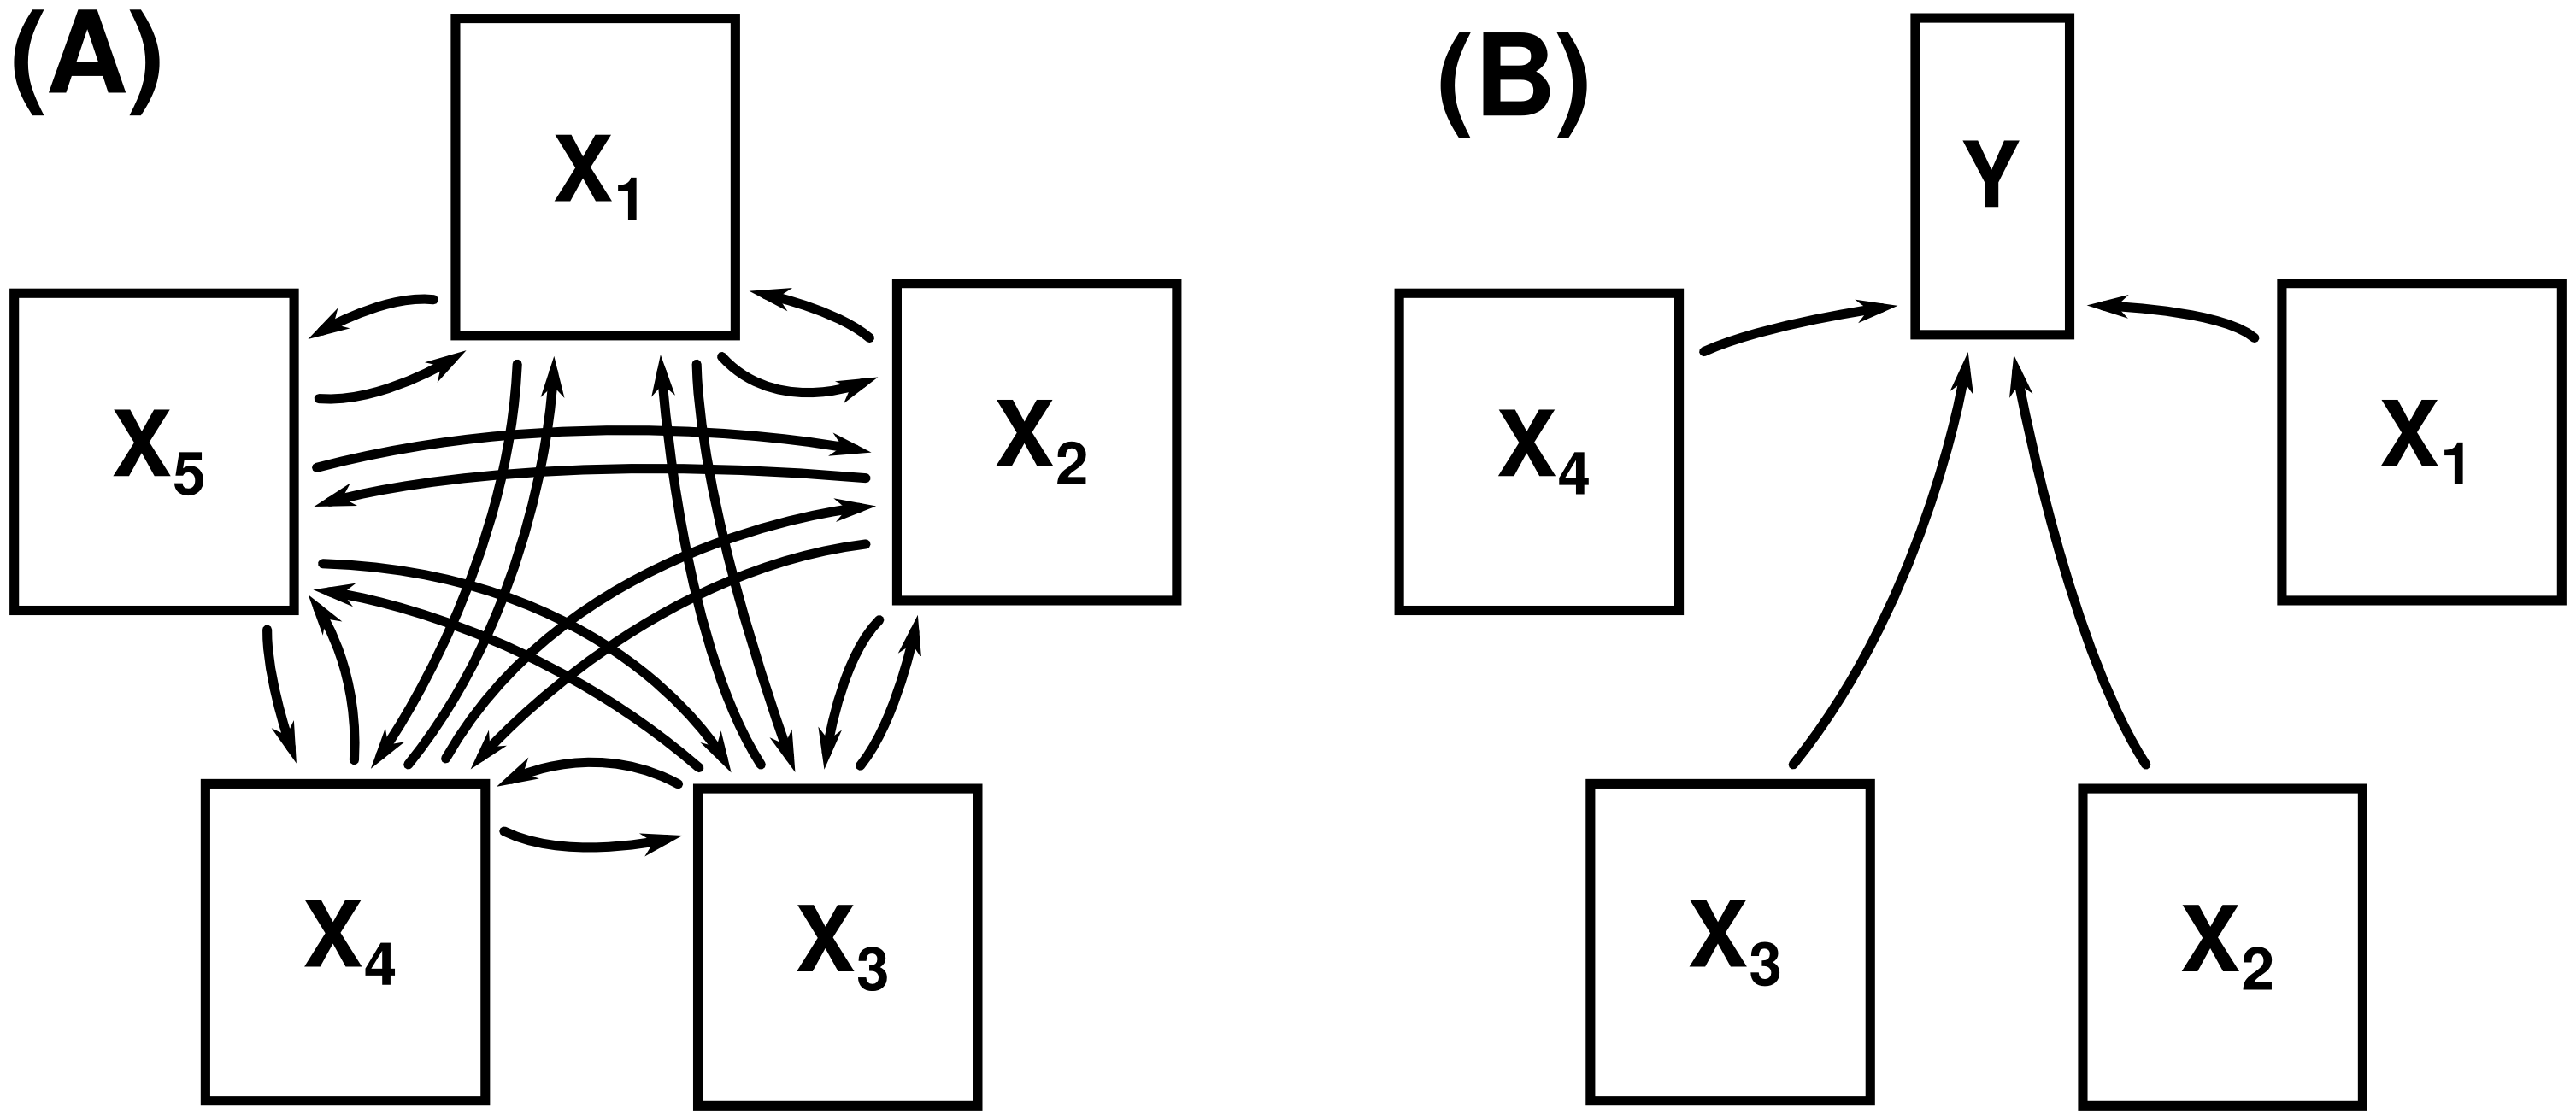
\includegraphics[width=3.5in]{figs/mva/13-assoc.png}
\caption
      [Association Graphs for OnPLS and MB-OPLS.]{
  {\bf Association Graphs for OnPLS and MB-OPLS.}
  \\
  ({\bf A}) Completely connected graph of nPLS and OnPLS regression
  models, in which no single matrix is considered unique.
  ({\bf B}) Sparsely connected acyclic graph of MB-PLS and MB-OPLS
  regression models, where each data block $\mathbf{X}_b$ predicts
  the unique matrix $\mathbf{Y}$.
}
\label{figure.3.13}
\end{SCfigure}

\begin{doublespace}
Computation of another predictive component requires the deflation of each
data block by both the predictive super-scores $\mathbf{t}$ and the
orthogonal super-scores $\mathbf{T_o}$, similar to the super-score deflation
method in MB-PLS \cite{westerhuis:jchemo1997}:
\begin{align}
\mathbf{X}_b' \gets& \: \mathbf{X}_b -
 \mathbf{t} {\mathbf{p}_b}^T -
 \mathbf{T_o} {\mathbf{P_o}_b}^T
 \quad \forall b \in \ints{1}{B} \\
\mathbf{Y} \gets& \: \mathbf{Y} - \mathbf{t} \mathbf{c}^T
\end{align}

In the same manner that block factors of CPCA-W and MB-PLS may be obtained from
PCA and PLS models -- respectively -- of the concatenated matrix of blocks
\cite{westerhuis:jchemo1998,smilde:jchemo2003}, MB-OPLS block scores and
loadings may be obtained from an OPLS model trained on the concatenated
matrix $\mathbf{X}$. The following algorithm describes the steps required
to extract block-level models from super-model scores and loadings.
\end{doublespace}

\begin{algorithm}[H]
\caption{Extraction of MB-OPLS Factors from OPLS}
\label{algorithm.3.7}
\begin{algorithmic}[1]
\REQUIRE $\mathbf{X}_b \in \mathbb{R}^{N \times K_b}
          \quad \forall b \in \ints{1}{B}$,%
       $\:\mathbf{Y} \in \mathbb{R}^{N \times M}$
\ENSURE $\mathbf{t} \in \mathbb{R}^N$,%
      $\:\mathbf{p} \in \mathbb{R}^K$,%
      $\:\mathbf{u} \in \mathbb{R}^N$,%
      $\:\mathbf{c} \in \mathbb{R}^M$,%
      $\:\mathbf{T_o} \in \mathbb{R}^{N \times a}$,%
      $\:\mathbf{P_o} \in \mathbb{R}^{K \times a}$, \\
      $\:\mathbf{t}_b \in \mathbb{R}^N$,%
      $\:\mathbf{p}_b \in \mathbb{R}^K$,%
      $\:\mathbf{T_o}_b \in \mathbb{R}^{N \times a}$,%
      $\:\mathbf{P_o}_b \in \mathbb{R}^{K \times a}
       \quad \forall b \in \ints{1}{B}$
\STATE $\{\mathbf{t}, \: \mathbf{p}, \: \mathbf{u}, \: \mathbf{c}, \:
        \mathbf{T_o}, \: \mathbf{P_o}\} \gets
        \mathrm{OPLS}(\mathbf{X}, \mathbf{Y})$
\FORALL{$b \in \ints{1}{B}$}
  \FORALL{$a_o \in \ints{1}{a}$}
    \STATE $\mathbf{t_o} \gets \mathbf{T_o}_{a_o}$ \COMMENT{
      Extract the $a_o$-th column of $\mathbf{T_o}$ }
    \STATE $\mathbf{w_o}_b \gets [\mathbf{W_o}_{a_o}]_b$ \COMMENT{
      Extract the $b$-th block of of $\mathbf{W_o}_{a_o}$ }
    \STATE $\mathbf{t_o}_b \gets \mathbf{X}_b \mathbf{w_o}_b$
    \STATE $\mathbf{p_o}_b \gets
            \tfrac{{\mathbf{X}_b}^T \mathbf{t_o}}
                  {\mathbf{t_o}^T \mathbf{t_o}}$
    \STATE $\mathbf{P_o}_b \gets [\mathbf{P_o}_b, \: \mathbf{p_o}_b]$
    \STATE $\mathbf{T_o}_b \gets [\mathbf{T_o}_b, \: \mathbf{t_o}_b]$
    \STATE $\mathbf{X}_b \gets \mathbf{X}_b - \mathbf{t_o} {\mathbf{p_o}_b}^T$
  \ENDFOR
  \STATE $\mathbf{w}_b \propto {\mathbf{X}_b}^T \mathbf{u}$
  \STATE $\mathbf{t}_b \gets \mathbf{X}_b \mathbf{w}_b$
  \STATE $\mathbf{p}_b \gets
          \tfrac{{\mathbf{X}_b}^T \mathbf{t}}
                {\mathbf{t}^T \mathbf{t}}$
  \STATE $\mathbf{X}_b \gets \mathbf{X}_b - \mathbf{t} {\mathbf{p}_b}^T$
\ENDFOR
\end{algorithmic}
\end{algorithm}

\begin{figure}[ht!]
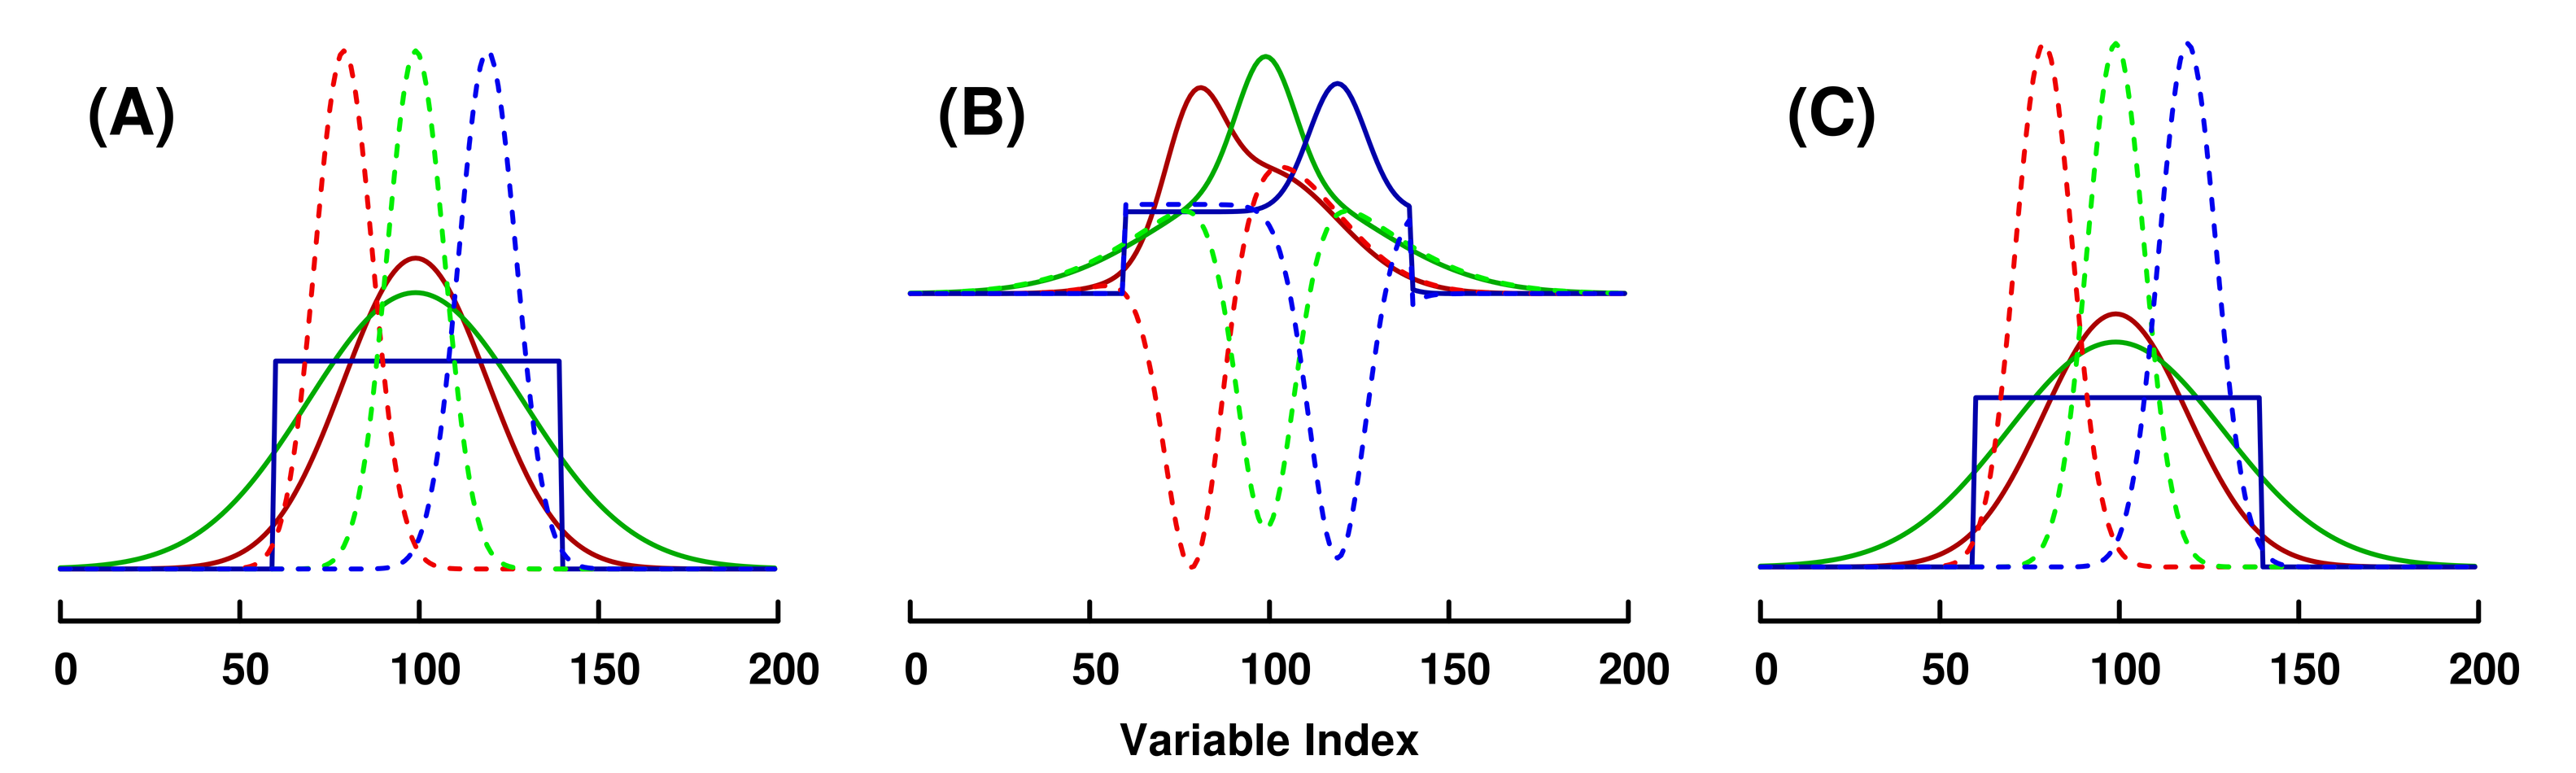
\includegraphics[width=6in]{figs/mva/14-mbopls.png}
\caption
      [Comparison of MB-PLS and MB-OPLS Loadings.]{
  {\bf Comparison of MB-PLS and MB-OPLS Loadings.}
  \\
  ({\bf A}) Original predictive (solid lines) and orthogonal (dashed lines)
  block loadings used to construct a toy three-block data structure having
  100 observations and 200 variables per block.
  ({\bf B}) Resulting MB-PLS block loadings from a two-component model,
  illustrating how the PLS algorithm mixes predictive information between
  multiple components in the presence of orthogonal variation.
  ({\bf C}) Resulting MB-OPLS predictive (solid) and orthogonal (dashed)
  block loadings from a one-component ($1+1$) model, effectively illustrating
  how MB-OPLS achieves the same segregation of predictive and orthogonal
  variation as OPLS and OnPLS on a per-block basis.
}
\label{figure.3.14}
\end{figure}

\begin{doublespace}
For each of the $B$ data blocks, the extraction procedure first computes
orthogonal block loadings and scores, and deflates them from the block. Then,
predictive block scores and loadings are computed using the method outlined
previously \cite{westerhuis:jchemo1998} for extracting MB-PLS block components
from a PLS model (steps 12--14). The resulting block scores and loadings from
algorithm 3.7 are identical to those produced by algorithm 3.6.
\end{doublespace}

\section{Validation}

\begin{figure}[ht!]
\includegraphics[width=6in]{figs/mva/15-overfit.png}
\caption
      [Demonstration of PLS Overfit Based on Variable Count.]{
  {\bf Demonstration of PLS Overfit Based on Variable Count.}
  \\
  ({\bf A}) Scores from a two-component PLS model of unit-variance scaled
  Gaussian white noise ($N = 10$, $K = 5$). Inset: \rsqy{} (blue) and \qsq{}
  (green) statistics for each component in the model, computed from 100
  iterations of seven-fold Monte Carlo cross-validation.
  ({\bf B}) Same scenario as ({\bf A}) with $K = 10$.
  ({\bf C}) Same scenario as ({\bf A}) with $K = 20$.
  ({\bf D}) Same scenario as ({\bf A}) with $K = 100$.
}
\label{figure.3.15}
\end{figure}

\begin{doublespace}
Application of the above bilinear factorization methods to one or more
spectral data matrices yields valuable insights into both general chemical
trends and relationships (e.g. from PCA) and response-predictive spectral
features (e.g. from OPLS) in those matrices. However, wanton use of these
multivariate methods without validation or knowledge of algorithmic intent
can quickly lead to statistically insignificant conclusions about the
underlying chemistry. The NIPALS-based algorithms described above are
highly numerically stable, even in the presence of multicollinearity,
noise, and missing data \cite{wold:cils2001,andersson:jchemo2009}. This
numerical stability almost guarantees that PCA, PLS and OPLS will return
a set of scores and loadings, even when those scores and loadings are only
based on a small fraction of the total variation in the data. PLS and OPLS
return biased regression coefficient estimates ($\hat{\mathbf{B}}_{PLS}$)
and force separation based on responses in scores space. OPLS is especially
adept at forcing scores-space separation, because its integrated OSC filter
removes systematic data matrix variation that does not ``agree'' with the
responses. These powerful modeling features make PLS and OPLS fully capable
of producing results based on noise alone, if so requested
\cite{westerhuis:metab2008a}. As the number of variables in the data increases
over the number of observations, the danger of overfitting also increases
(\figref{3.15}{Figure 3.15}). In effect, the probability of observing
correlations to the responses increases with variable count, just as the
probability of observing long runs of heads or tails increases with the number
of fair coin tosses.
\\\\
In chemometric studies of spectroscopic datasets, where $N \ll K$, the tendency
of bilinear models to over-fit must be balanced by rigorous application of
several validation methods. When sufficient validation is lacking, any
conclusions drawn from these models should automatically be treated as
suspect from a statistical viewpoint. Therefore, all efforts must be taken
during experimental design, data collection and handling in order to obtain
data and models that acceptably withstand cross-validation.
\end{doublespace}

\subsection{Explained Variation}

\begin{doublespace}
In general, the amount of variation explained by a bilinear factorization of
a matrix is quantified by its sum of squares:
\begin{equation*}
SS \left\{ \mathbf{t} \mathbf{p}^T \right\} = \frosq{\mathbf{t} \mathbf{p}^T}
\end{equation*}
where $\frosq{\cdot}$ denotes the squared Frobenius norm, which will be used
as a shorthand for the sum of squares. Because the raw sum of squares is not
scale-invariant, it is normally reported as a ratio relative to the total sum
of squares. In the context of a PCA (equation 3.20), this ratio is referred
to as \rsqx{} (or simply \rsq{}):
\begin{align}
R^2_X
 =& \: \frac{\ssfit{}}{\sstot{}}
     = \frac{\frosq{\mathbf{T} \mathbf{P}^T}}{\frosq{\mathbf{X}}} \\
 =& \: 1 - \frac{\sserr{}}{\sstot{}}
     = 1 - \frac{\frosq{\mathbf{E}}}{\frosq{\mathbf{X}}}
\end{align}
where the second set of equalities arises from the fact that PCA loadings are
eigenvectors of $\mathbf{X}^T \mathbf{X}$ and right singular vectors of
$\mathbf{X}$ \cite{jolliffe2002}. The cumulative \rsqx{} statistic may be
broken into sums of per-component \rsqx{} statistics, due to the orthonormality
properties of principal components:
\begin{equation}
R^2_X =
 \sum_{a=1}^A
 \frac{\frosq{\mathbf{t}_a {\mathbf{p}_a}^T}}
      {\frosq{\mathbf{X}}}
\end{equation}

In the case of PLS modeling (equation 3.37), a second ratio exists (\rsqy{})
that quantifies the amount of variation explained in the responses:
\begin{align}
R^2_Y
 =& \: \frac{\frosq{\mathbf{T} \mathbf{C}^T}}{\frosq{\mathbf{Y}}} \\
 =& \: 1 - \frac{\frosq{\mathbf{F}}}{\frosq{\mathbf{Y}}}
\end{align}

Similar expressions exist for the predictive and orthogonal factorizations of
$\mathbf{X}$ in OPLS models, which are referred to as \rsqxp{} and \rsqxo{},
respectively. While these \rsq{} statistics provide valuable first insights
into the amount of variation that may be explained by a multivariate model,
they are gross over-estimations of model reliability and should not be used
during model selection as a means of determining the optimal component count,
$A^\ast$. Cross-validatory methods discussed in later sections provide more
effective means of identifying $A^\ast$ during model training.
\end{doublespace}

\subsection{External Cross-validation}

\begin{doublespace}
In its most traditional form, cross-validation involves the division of $N$
observations in a dataset (i.e. $\mathbf{X}$ and $\mathbf{Y}$) into a training
set ($\mathbf{X}_t$ and $\mathbf{Y}_t$) having $N_t$ observations and a
validation set ($\mathbf{X}_v$ and $\mathbf{Y}_v$) having $N_v$ observations.
The training and validation datasets are then processed and treated separately
using identical methods, and models are constructed on the training dataset.
In the case of PLS modeling, the analyst will arrive at the following equation:
\begin{equation}
\mathbf{Y}_t = \mathbf{X}_t \mathbf{W}^\ast \mathbf{C}^T + \mathbf{F}
\end{equation}

Assessment of model reliability is then performed by estimating the responses
of the validation dataset using the trained model, like so:
\begin{equation}
\hat{\mathbf{Y}}_v = \mathbf{X}_v \mathbf{W}^\ast \mathbf{C}^T
\end{equation}
where the predicted residual sum of squares (PRESS) statistic is now readily
computable from the sum of squares of the difference between true and estimated
validation-set responses:
\begin{equation}
\mathrm{PRESS} = \frosq{\mathbf{Y}_v - \hat{\mathbf{Y}}_v}
\end{equation}

Like any other sum of squares measure, PRESS depends on the magnitudes of the
values in $\mathbf{Y}$. Thus, a scale-invariant reporter of reliability
(\qsq{}) is obtained from the PRESS statistic as follows:
\begin{equation}
Q^2
 = 1 - \frac{\mathrm{PRESS}}{\sstot{}}
 = 1 - \frac{\frosq{\mathbf{Y}_v - \hat{\mathbf{Y}}_v}}{\frosq{\mathbf{Y}_v}}
\end{equation}

This model reliability statistic is often referred to as a ``cross-validated''
\rsq{} statistic, and provides a relative measure of how well a given model
will generalize to the estimation of future observations. Like \rsq{}
statistics, \qsq{} is also computable on a per-component basis.
\\\\
When the values in $\mathbf{Y}$ do not vary continuously, but instead hold
binary class membership information, it is possible for \qsq{} -- as defined
by the previous equation -- to under-estimate model reliability
\cite{westerhuis:metab2008b}. In the case of two-class discrimination, \qsq{}
quadratically penalizes values in $\hat{\mathbf{y}}$ that are beyond the class
labels in $\mathbf{y}$. In more concrete terms, a cross-validation predicted
class label of 1.5 for a true class label of 1.0 should incur no penalty, as
it represents an unambiguous prediction. However, the quadratic nature of
\qsq{} penalizes such results. When PLS and OPLS are used for binary class
discrimination, the more suitable ``discriminant \qsq{}'' (\dqsq{}) is a more
suitable metric of reliability:
\begin{equation}
DQ^2 = 1 - \frac{\mathrm{PRESSD}}{\sstot{}}
\end{equation}
where PRESSD represents the discriminant PRESS statistic:
\begin{equation}
\mathrm{PRESSD} = \sum_{n=1}^N
\begin{cases}
  0 & \text{if } y_n = 1 \text{ and } \hat{y}_n > 1 \\
  0 & \text{if } y_n = 0 \text{ and } \hat{y}_n < 0 \\
  (y_n - \hat{y}_n)^2 & \text{else}
\end{cases}
\end{equation}

In effect, PRESSD computes the sum of all squared $\mathbf{y}$-residuals that
represent a potentially ambiguous classification \cite{westerhuis:metab2008b}.
The same result may be achieved by appropriately bounding the values within
$\hat{\mathbf{y}}$ to the class label extents in $\mathbf{y}$, followed by the
use of standard PRESS and \qsq{} calculations. This alternative strategy has
the added benefit of ensuring that the prediction sum of squares
$\frosq{\hat{\mathbf{y}}}$ never exceeds the total sum of squares
$\frosq{\mathbf{y}}$, which is a requirement for CV-ANOVA, discussed below.
\end{doublespace}

\subsection{Internal Cross-validation}

\subsubsection{Supervised Models}

\begin{doublespace}
Due to the severely limited number of observations in most chemometric studies,
the practice of external cross-validation is rare, and all observations are
usually retained for model training. Nevertheless, model reliability statistics
may be obtained from the similar practice of \emph{internal} cross-validation.
In any internal cross-validation scheme, the $N$ observations of a given
dataset are divided into $G$ groups, referred to as $G$-fold or
leave-$n$-out cross-validation (where $n = \lfloor N / G \rfloor$). Each
group is then left out in turn, and its responses are estimated from a model
trained on the remainder of the data. To more succinctly introduce internal
cross-validation procedures, the set of all partitionings of $N$ elements into
$G$ groups, denoted $\mathbb{P}(N, G)$, shall be introduced:
\begin{equation}
\mathbb{P}(N, G) \equiv \big\{
 \mathbf{p} \mid \mathbf{p} \in \mathbb{Z}^N
 \wedge
 1 \le p_n \le G
 \quad \forall n \in \ints{1}{N}
\big\}
\end{equation}

As an example, one member of the set $\mathbb{P}(7, 3)$ is
$(1,2,3,1,2,3,1)$.\footnote{This type of partitioning actually has a name, and
is often seen in practical cross-validation schemes. It is colloquially
referred to as a ``Venetian blinds'' partitioning of seven observations into
three groups.} Given a partitioning $\boldsymbol{\sigma} \in \mathbb{P}(N, G)$,
the following algorithm demonstrates the computation of \qsq{} for a single
PLS component:
\end{doublespace}

\begin{algorithm}[H]
\caption{Internal PLS Component Cross-validation}
\label{algorithm.3.8}
\begin{algorithmic}[1]
\REQUIRE $\mathbf{X} \in \mathbb{R}^{N \times K}$,%
       $\:\mathbf{Y} \in \mathbb{R}^{N \times M}$,%
       $\:G$, $\:\boldsymbol{\sigma} \in \mathbb{P}(N, G)$
\ENSURE $Q^2 \in \mathbb{R}$
\FORALL{$g \in \ints{1}{G}$}
  \STATE $n_g \gets \{ n \mid n \in \ints{1}{N} \wedge \sigma_n = g \}$
  \STATE $\{\mathbf{t}, \mathbf{p}, \mathbf{u}, \mathbf{c}, \mathbf{w}\}
          \gets \mathrm{PLS}(\mathbf{X}^{(-n_g)},
                             \mathbf{Y}^{(-n_g)})$ \COMMENT{
 $\mathbf{X}^{(-n_g)}$, $\mathbf{Y}^{(-n_g)}$ contain no rows from group $g$
}
  \STATE $\mathbf{B}^{(n_g)} \gets \tfrac{\mathbf{w} \mathbf{c}^T}
                                         {\mathbf{p}^T \mathbf{w}}$
\ENDFOR
\FORALL{$n \in \ints{1}{N}$}
  \STATE $\hat{\mathbf{y}}_n \gets
          \mathbf{x}_n \mathbf{B}^{(\sigma_n)}$ \COMMENT{
 $\hat{\mathbf{y}}_n$, $\mathbf{x}_n$ are the $n$-th rows of
 $\hat{\mathbf{Y}}$, $\mathbf{X}$
}
\ENDFOR
\STATE $Q^2 \gets 1 - \frac{\frosq{\mathbf{Y} - \hat{\mathbf{Y}}}}
                           {\frosq{\mathbf{Y}}}$
\end{algorithmic}
\end{algorithm}

\begin{doublespace}
In the simplest case where $G = N$, known as leave-one-out cross-validation
(LOOCV), only one observation is left out at a time. It has been shown,
however, that leave-one-out methods do not identify optimal models as
effectively as leave-$n$-out methods as $N$ increases \cite{shao:jasa1993},
so $G$ should be less than the number of observations whenever possible.
Within a leave-$n$-out cross-validation of $N$ observations, there are
$\binom{N}{n}$ different ways to partition the dataset into the desired
number of groups. A complete cross-validation would require the evaluation
of all possible partitions, which is computationally intractable even for
small (e.g. $N \ge 20$) datasets. While it is possible to arbitrarily select
a single partitioning, such as a regular pattern of group assignment, it is
much more attractive to randomly resample a number of partitionings ($n_p$)
from the set of $\binom{N}{n}$ possibilities
($\boldsymbol{\sigma} \sim \mathbb{P}(N,G)$) in a
Monte Carlo leave-$n$-out cross-validation approach \cite{xu:cils2001}. Monte
Carlo cross-validation offers the possibility of assigning confidence regions
to reported \qsq{} values for a given dataset, which provides the analyst with
further information on model reliability estimates.
\\\\
In practice, per-component \qsq{} statistics provide a means of determining
$A^\ast$, the optimal component count. When new components are added to the
model that fail to reliably estimate the responses under cross-validation,
their \qsq{} values will become negative. Thus, a practical rule during model
training is to only retain components having positive \qsq{} statistics.
\end{doublespace}

\begin{figure}[ht!]
\begin{center}
  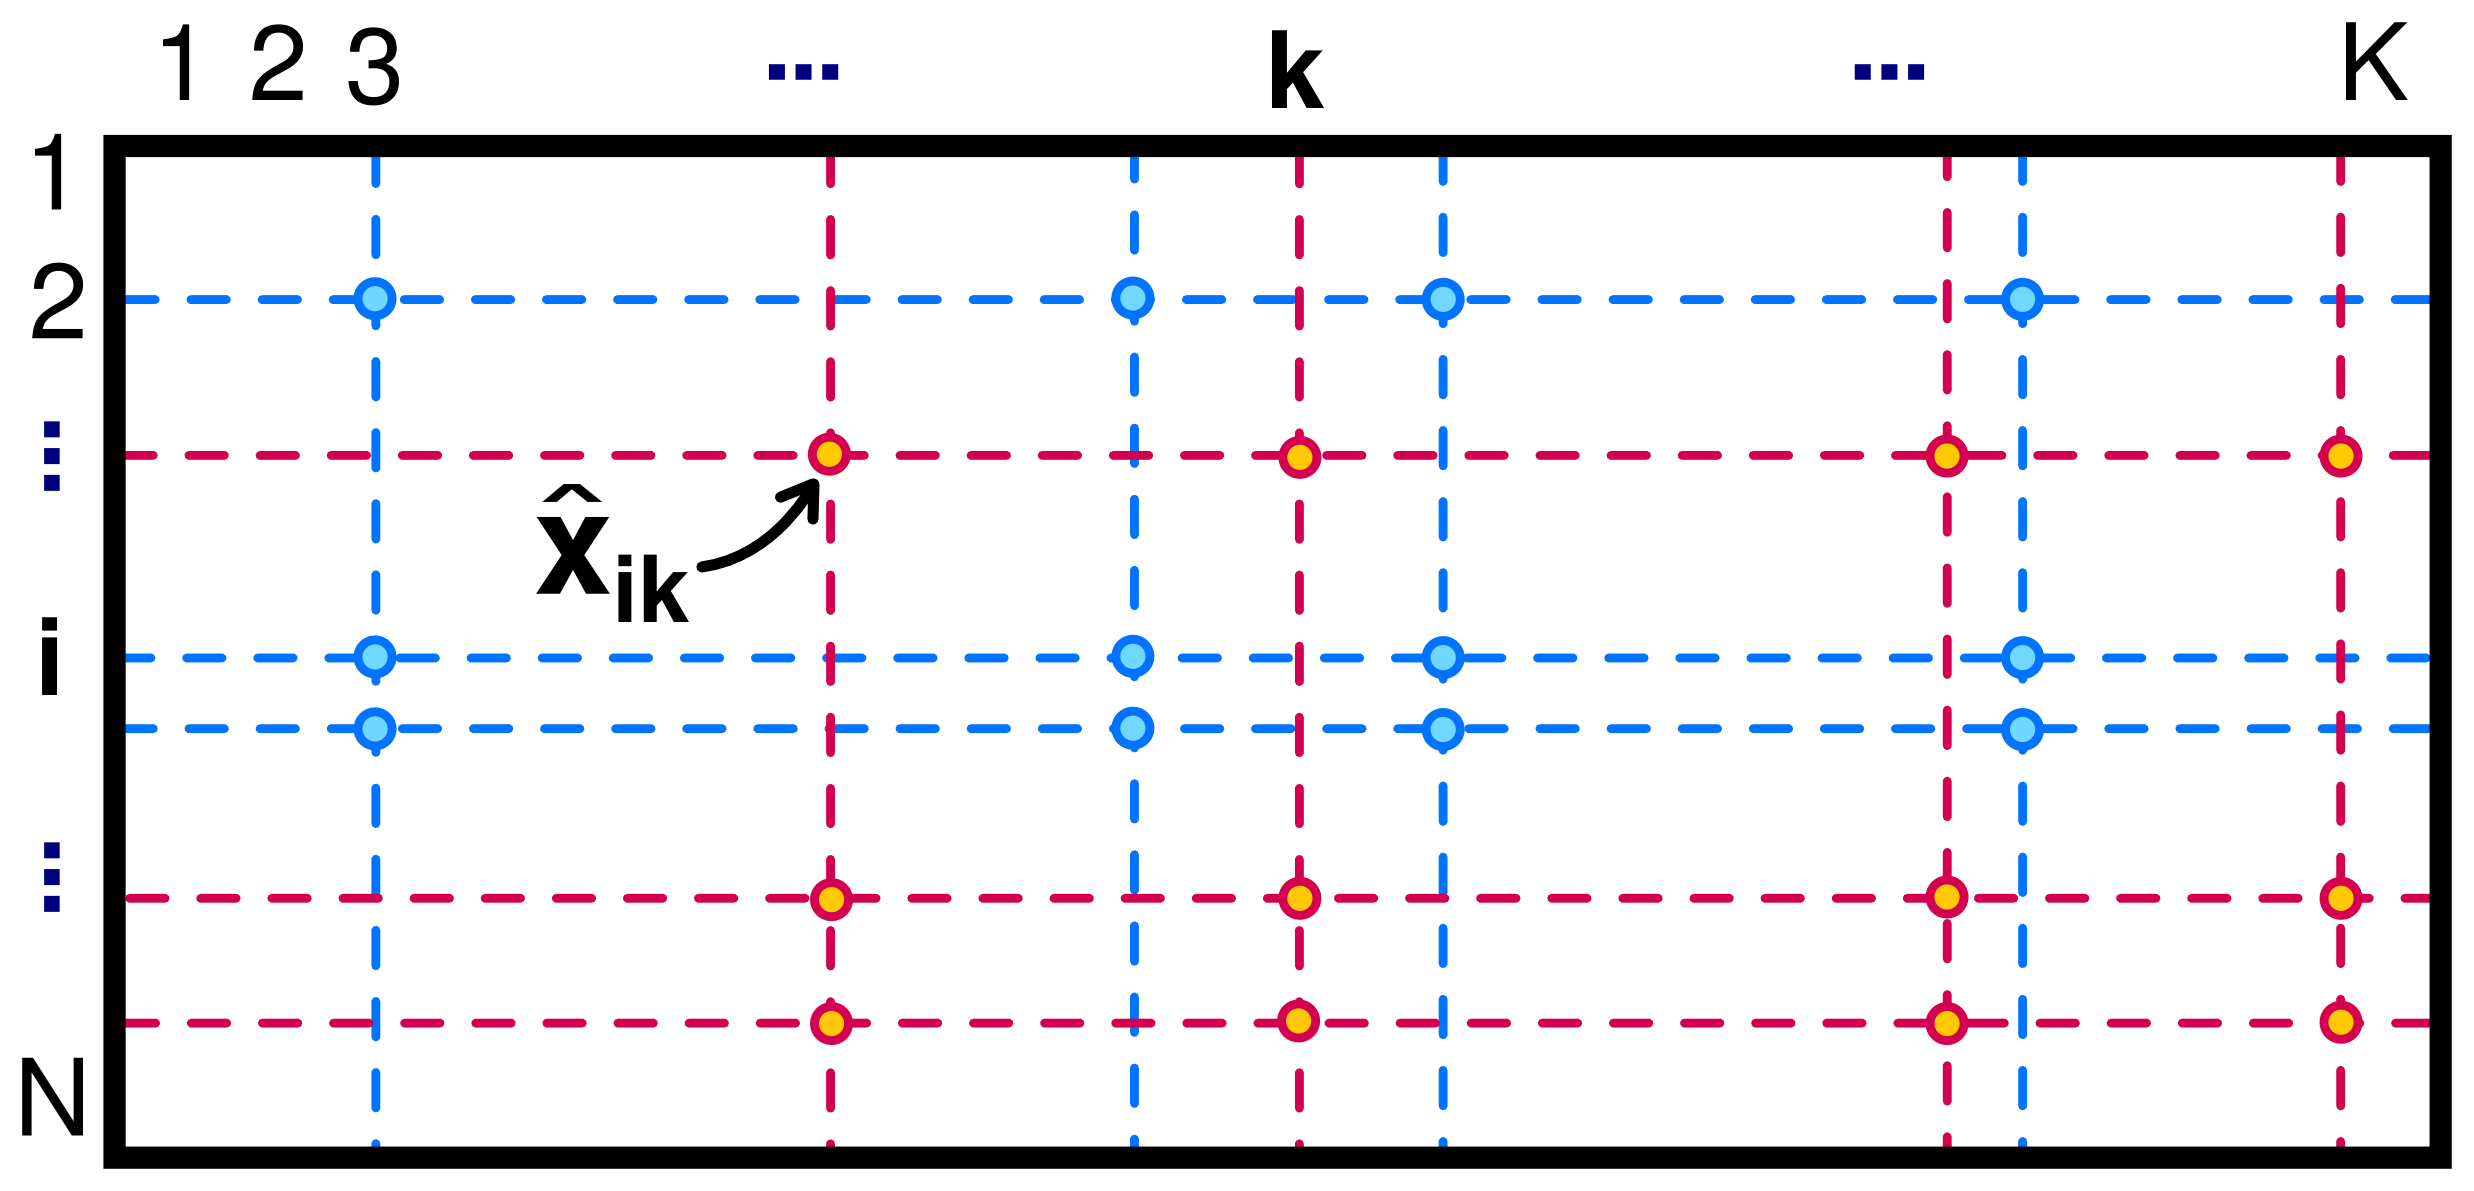
\includegraphics[width=4in]{figs/mva/16-pcacv.png}
\end{center}
\caption
      [Partitioning in Leave-$n$-out PCA Cross-validation.]{
  {\bf Partitioning in Leave-$n$-out PCA Cross-validation.}
  \\
  Graphical illustration of two different partitionings (red and blue) of a
  data matrix. Each partitioning (group) requires the computation of a set of
  scores ($\hat{\mathbf{t}}$) and loadings ($\hat{\mathbf{p}}$) in order to
  estimate it's left-out values, indicated by filled circles. Estimation of
  $\hat{x}_{ik}$ requires computation of $\hat{\mathbf{t}}$ with variable $k$
  left out and $\hat{\mathbf{p}}$ with observation $i$ left out. The value of
  $\hat{x}_{ik}$ is then obtained from the $(i,k)$-th index of
  $\hat{\mathbf{t}} \hat{\mathbf{p}}^T$
}
\label{figure.3.16}
\end{figure}

\subsubsection{Unsupervised Models}

\begin{doublespace}
Internal cross-validation of unsupervised PCA models poses a unique challenge
in comparison to PLS and OPLS, as it does not involve the prediction of a set
of responses \cite{eastment:tech1982,krzanowski:biom1987,eshghi:cils2014}.
Eshghi \cite{eshghi:cils2014} provides a more comprehensive review of internal
cross-validation practices for PCA models. In short, leave-$n$-out
cross-validation of PCA models requires that both observations \emph{and}
variables be partitioned into $G$ groups. The resulting pair of partitionings
allows groups of data matrix elements to be left out and recomputed during
cross-validation. For each group, a score vector $\hat{\mathbf{t}}$ is
computed after leaving out variables in the group, and a loading vector
$\hat{\mathbf{p}}$ is computed after leaving out observations in the group.
The outer product of $\hat{\mathbf{t}}$ and $\hat{\mathbf{p}}$ is then used
in estimating the data matrix elements located at the intersections of the
left-out variables and observations (\figref{3.16}{Figure 3.16}). The
following algorithm demonstrates the computation of \qsq{} for a single
principal component, given a row partitioning $\boldsymbol{\sigma}$ and
a column partitioning $\boldsymbol{\rho}$:
\end{doublespace}

\begin{algorithm}[H]
\caption{Internal PCA Component Cross-validation}
\label{algorithm.3.9}
\begin{algorithmic}[1]
\REQUIRE $\mathbf{X} \in \mathbb{R}^{N \times K}$, $\:G$,
       $\:\boldsymbol{\sigma} \in \mathbb{P}(N, G)$,%
       $\:\boldsymbol{\rho} \in \mathbb{P}(K, G)$
\ENSURE $Q^2 \in \mathbb{R}$
\FORALL{$g_1 \in \ints{1}{G}$}
  \STATE $n_g \gets \{ n \mid n \in \ints{1}{N} \wedge \sigma_n = g_1 \}$
    \STATE $\hat{\mathbf{p}} \gets \mathrm{PCA}(\mathbf{X}^{(-n_g)})$ \COMMENT{
    $\mathbf{X}^{(-n_g)}$ contains no rows from group $g$}

  \FORALL{$g_2 \in \ints{1}{G}$}
    \STATE $k_g \gets \{ k \mid k \in \ints{1}{K} \wedge \rho_k = g_2 \}$
    \STATE $\hat{\mathbf{t}} \gets \mathrm{PCA}(\mathbf{X}^{(-k_g)})$ \COMMENT{
    $\mathbf{X}^{(-k_g)}$ contains no columns from group $g$}
    \STATE $\hat{\mathbf{t}} \gets \hat{\mathbf{t}}
            \sqrt{\tfrac{K}{K - |k_g|}}$
    \FORALL{$n \in n_g$}
      \FORALL{$k \in k_g$}
        \STATE $\hat{\mathbf{X}}_{n,k} \gets
                \hat{\mathbf{t}}_n \hat{\mathbf{p}}_k$
      \ENDFOR
    \ENDFOR
  \ENDFOR
\ENDFOR
\STATE $Q^2 \gets 1 - \frac{\frosq{\mathbf{X} - \hat{\mathbf{X}}}}
                           {\frosq{\mathbf{X}}}$
\end{algorithmic}
\end{algorithm}

\subsection{Response Permutation Testing}

\begin{doublespace}
While internal cross-validation metrics such as \qsq{}, number of
misclassifications, and AUROC \cite{westerhuis:metab2008a} are a good first
insight into model reliability, they do not provide a robust mechanism for
discriminating between low- and high-quality models. Methods that report a
degree of statistical significance in the form of a $p$ value are preferred,
as they may be compared to a threshold (e.g. $\alpha = 0.05$). One such method,
known as response permutation testing, establishes a distribution of models
representing the null hypothesis ($H_0$) that no relationship exists between
the data and responses \cite{westerhuis:metab2008a}. For a number of
iterations, the rows of the response matrix $\mathbf{Y}$ are randomly permuted
to yield a null response matrix $\tilde{\mathbf{Y}}$, upon which a supervised
PLS or OPLS model is trained. The set of models generated after response
permutation -- more specifically their \rsq{} and \qsq{} parameters -- may be
compared against those of the original model to obtain a $p$ value. Provided
the resulting $p$ value is less than the defined threshold $\alpha$, the
analyst may reject the null hypothesis that the original model is based on
random correlations between $\mathbf{X}$ and $\mathbf{Y}$.
\end{doublespace}

\subsection{CV-ANOVA Testing}

\begin{doublespace}
Response permutation testing capably reports $p$ values via hypothesis testing
of model reliability, but it requires significant computation time to train
the 100 -- 1,000 models required for an accurate result. The alternative
CV-ANOVA testing method effectively requires no additional computation time
after internal cross-validation, as it compares the fitted $\mathbf{Y}$
residuals obtained from cross-validation procedures \cite{eriksson:jchemo2008}.
In effect, CV-ANOVA tests whether the mean square error of fitted residuals
from PLS and OPLS models is significantly smaller than the total mean square
variation in $\hat{\mathbf{Y}}$. By comparing the ratio of these mean square
values to an $F$ distribution, CV-ANOVA reports its own $p$ value which may
again be compared to a predefined threshold.
\end{doublespace}

\section{Conclusions}

\begin{doublespace}
Multivariate bilinear factorizations such as PCA, PLS and OPLS provide an
essential platform for rapid information extraction of rich spectral datasets.
Through proper application of processing and treatment, optimal choice of
modeling algorithms, and judicious administration of validation metrics,
multivariate analysis can lend a powerful hand in biochemical examination of
complex, multiparametric metabolic systems. Specific applications of
multivariate analysis in metabolomics are discussed in further detail in the
following chapter.
\end{doublespace}

\bibliographystyle{abbrv}
\bibliography{bworley}

